\documentclass[1p]{elsarticle_modified}
%\bibliographystyle{elsarticle-num}

%\usepackage[colorlinks]{hyperref}
%\usepackage{abbrmath_seonhwa} %\Abb, \Ascr, \Acal ,\Abf, \Afrak
\usepackage{amsfonts}
\usepackage{amssymb}
\usepackage{amsmath}
\usepackage{amsthm}
\usepackage{scalefnt}
\usepackage{amsbsy}
\usepackage{kotex}
\usepackage{caption}
\usepackage{subfig}
\usepackage{color}
\usepackage{graphicx}
\usepackage{xcolor} %% white, black, red, green, blue, cyan, magenta, yellow
\usepackage{float}
\usepackage{setspace}
\usepackage{hyperref}

\usepackage{tikz}
\usetikzlibrary{arrows}

\usepackage{multirow}
\usepackage{array} % fixed length table
\usepackage{hhline}

%%%%%%%%%%%%%%%%%%%%%
\makeatletter
\renewcommand*\env@matrix[1][\arraystretch]{%
	\edef\arraystretch{#1}%
	\hskip -\arraycolsep
	\let\@ifnextchar\new@ifnextchar
	\array{*\c@MaxMatrixCols c}}
\makeatother %https://tex.stackexchange.com/questions/14071/how-can-i-increase-the-line-spacing-in-a-matrix
%%%%%%%%%%%%%%%

\usepackage[normalem]{ulem}

\newcommand{\msout}[1]{\ifmmode\text{\sout{\ensuremath{#1}}}\else\sout{#1}\fi}
%SOURCE: \msout is \stkout macro in https://tex.stackexchange.com/questions/20609/strikeout-in-math-mode

\newcommand{\cancel}[1]{
	\ifmmode
	{\color{red}\msout{#1}}
	\else
	{\color{red}\sout{#1}}
	\fi
}

\newcommand{\add}[1]{
	{\color{blue}\uwave{#1}}
}

\newcommand{\replace}[2]{
	\ifmmode
	{\color{red}\msout{#1}}{\color{blue}\uwave{#2}}
	\else
	{\color{red}\sout{#1}}{\color{blue}\uwave{#2}}
	\fi
}

\newcommand{\Sol}{\mathcal{S}} %segment
\newcommand{\D}{D} %diagram
\newcommand{\A}{\mathcal{A}} %arc


%%%%%%%%%%%%%%%%%%%%%%%%%%%%%5 test

\def\sl{\operatorname{\textup{SL}}(2,\Cbb)}
\def\psl{\operatorname{\textup{PSL}}(2,\Cbb)}
\def\quan{\mkern 1mu \triangleright \mkern 1mu}

\theoremstyle{definition}
\newtheorem{thm}{Theorem}[section]
\newtheorem{prop}[thm]{Proposition}
\newtheorem{lem}[thm]{Lemma}
\newtheorem{ques}[thm]{Question}
\newtheorem{cor}[thm]{Corollary}
\newtheorem{defn}[thm]{Definition}
\newtheorem{exam}[thm]{Example}
\newtheorem{rmk}[thm]{Remark}
\newtheorem{alg}[thm]{Algorithm}

\newcommand{\I}{\sqrt{-1}}
\begin{document}

%\begin{frontmatter}
%
%\title{Boundary parabolic representations of knots up to 8 crossings}
%
%%% Group authors per affiliation:
%\author{Yunhi Cho} 
%\address{Department of Mathematics, University of Seoul, Seoul, Korea}
%\ead{yhcho@uos.ac.kr}
%
%
%\author{Seonhwa Kim} %\fnref{s_kim}}
%\address{Center for Geometry and Physics, Institute for Basic Science, Pohang, 37673, Korea}
%\ead{ryeona17@ibs.re.kr}
%
%\author{Hyuk Kim}
%\address{Department of Mathematical Sciences, Seoul National University, Seoul 08826, Korea}
%\ead{hyukkim@snu.ac.kr}
%
%\author{Seokbeom Yoon}
%\address{Department of Mathematical Sciences, Seoul National University, Seoul, 08826,  Korea}
%\ead{sbyoon15@snu.ac.kr}
%
%\begin{abstract}
%We find all boundary parabolic representation of knots up to 8 crossings.
%
%\end{abstract}
%\begin{keyword}
%    \MSC[2010] 57M25 
%\end{keyword}
%
%\end{frontmatter}

%\linenumbers
%\tableofcontents
%
\newcommand\colored[1]{\textcolor{white}{\rule[-0.35ex]{0.8em}{1.4ex}}\kern-0.8em\color{red} #1}%
%\newcommand\colored[1]{\textcolor{white}{ #1}\kern-2.17ex	\textcolor{white}{ #1}\kern-1.81ex	\textcolor{white}{ #1}\kern-2.15ex\color{red}#1	}

{\Large $\underline{12a_{0340}~(K12a_{0340})}$}

\setlength{\tabcolsep}{10pt}
\renewcommand{\arraystretch}{1.6}
\vspace{1cm}\begin{tabular}{m{100pt}>{\centering\arraybackslash}m{274pt}}
\multirow{5}{120pt}{
	\centering
	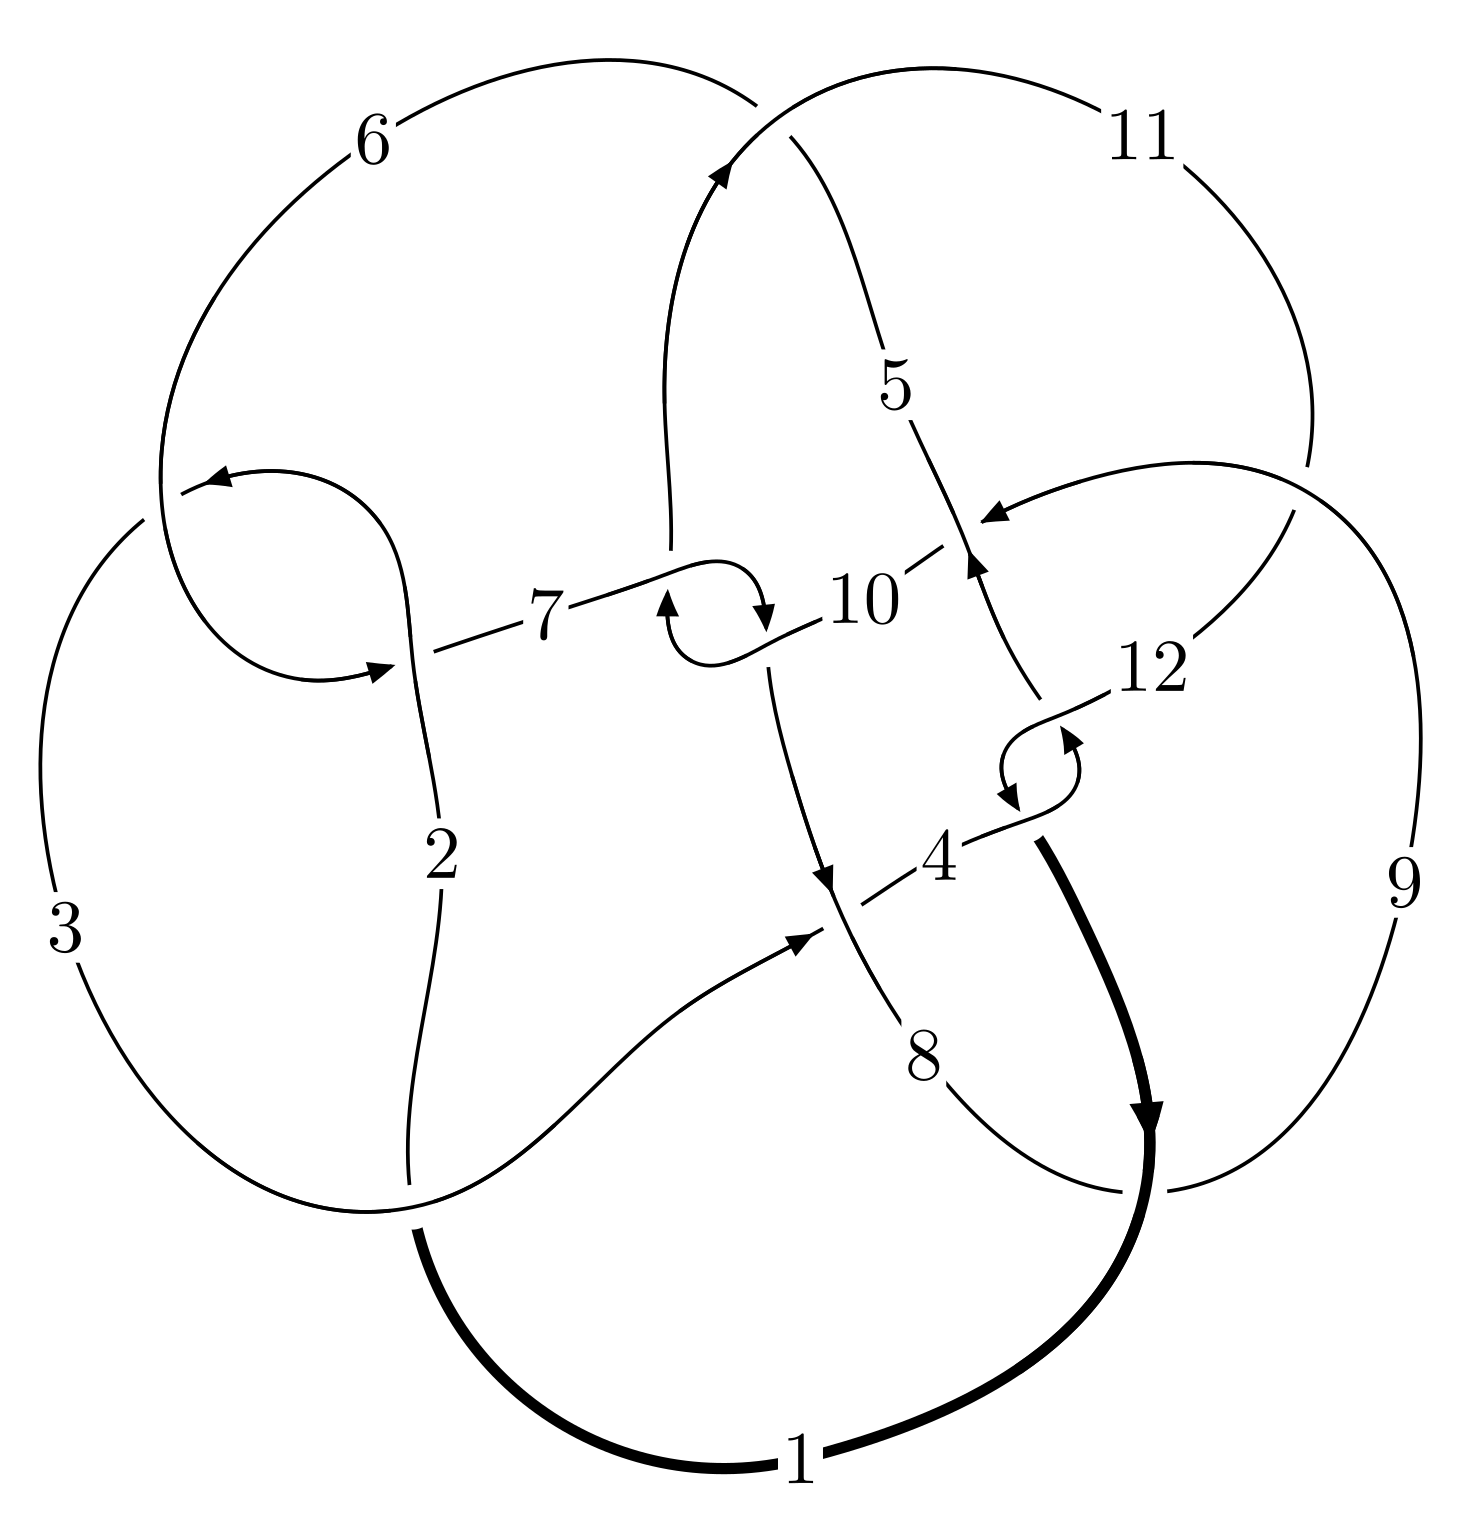
\includegraphics[width=112pt]{../../../GIT/diagram.site/Diagrams/png/1141_12a_0340.png}\\
\ \ \ A knot diagram\footnotemark}&
\allowdisplaybreaks
\textbf{Linearized knot diagam} \\
\cline{2-2}
 &
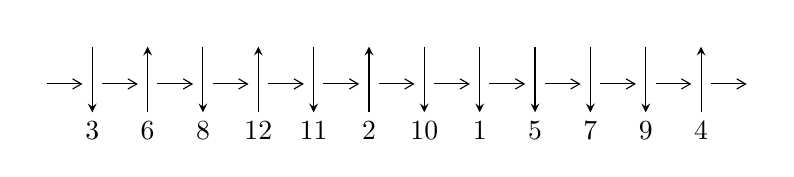
\begin{tikzpicture}[x=20pt, y=17pt]
	% nodes
	\node (C0) at (0, 0) {};
	\node (C1) at (1, 0) {};
	\node (C1U) at (1, +1) {};
	\node (C1D) at (1, -1) {3};

	\node (C2) at (2, 0) {};
	\node (C2U) at (2, +1) {};
	\node (C2D) at (2, -1) {6};

	\node (C3) at (3, 0) {};
	\node (C3U) at (3, +1) {};
	\node (C3D) at (3, -1) {8};

	\node (C4) at (4, 0) {};
	\node (C4U) at (4, +1) {};
	\node (C4D) at (4, -1) {12};

	\node (C5) at (5, 0) {};
	\node (C5U) at (5, +1) {};
	\node (C5D) at (5, -1) {11};

	\node (C6) at (6, 0) {};
	\node (C6U) at (6, +1) {};
	\node (C6D) at (6, -1) {2};

	\node (C7) at (7, 0) {};
	\node (C7U) at (7, +1) {};
	\node (C7D) at (7, -1) {10};

	\node (C8) at (8, 0) {};
	\node (C8U) at (8, +1) {};
	\node (C8D) at (8, -1) {1};

	\node (C9) at (9, 0) {};
	\node (C9U) at (9, +1) {};
	\node (C9D) at (9, -1) {5};

	\node (C10) at (10, 0) {};
	\node (C10U) at (10, +1) {};
	\node (C10D) at (10, -1) {7};

	\node (C11) at (11, 0) {};
	\node (C11U) at (11, +1) {};
	\node (C11D) at (11, -1) {9};

	\node (C12) at (12, 0) {};
	\node (C12U) at (12, +1) {};
	\node (C12D) at (12, -1) {4};
	\node (C13) at (13, 0) {};

	% arrows
	\draw[->,>={angle 60}]
	(C0) edge (C1) (C1) edge (C2) (C2) edge (C3) (C3) edge (C4) (C4) edge (C5) (C5) edge (C6) (C6) edge (C7) (C7) edge (C8) (C8) edge (C9) (C9) edge (C10) (C10) edge (C11) (C11) edge (C12) (C12) edge (C13) ;	\draw[->,>=stealth]
	(C1U) edge (C1D) (C2D) edge (C2U) (C3U) edge (C3D) (C4D) edge (C4U) (C5U) edge (C5D) (C6D) edge (C6U) (C7U) edge (C7D) (C8U) edge (C8D) (C9U) edge (C9D) (C10U) edge (C10D) (C11U) edge (C11D) (C12D) edge (C12U) ;
	\end{tikzpicture} \\
\hhline{~~} \\& 
\textbf{Solving Sequence} \\ \cline{2-2} 
 &
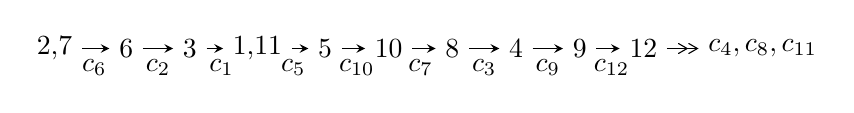
\begin{tikzpicture}[x=23pt, y=7pt]
	% node
	\node (A0) at (-1/8, 0) {2,7};
	\node (A1) at (1, 0) {6};
	\node (A2) at (2, 0) {3};
	\node (A3) at (49/16, 0) {1,11};
	\node (A4) at (33/8, 0) {5};
	\node (A5) at (41/8, 0) {10};
	\node (A6) at (49/8, 0) {8};
	\node (A7) at (57/8, 0) {4};
	\node (A8) at (65/8, 0) {9};
	\node (A9) at (73/8, 0) {12};
	\node (C1) at (1/2, -1) {$c_{6}$};
	\node (C2) at (3/2, -1) {$c_{2}$};
	\node (C3) at (5/2, -1) {$c_{1}$};
	\node (C4) at (29/8, -1) {$c_{5}$};
	\node (C5) at (37/8, -1) {$c_{10}$};
	\node (C6) at (45/8, -1) {$c_{7}$};
	\node (C7) at (53/8, -1) {$c_{3}$};
	\node (C8) at (61/8, -1) {$c_{9}$};
	\node (C9) at (69/8, -1) {$c_{12}$};
	\node (A10) at (11, 0) {$c_{4},c_{8},c_{11}$};

	% edge
	\draw[->,>=stealth]	
	(A0) edge (A1) (A1) edge (A2) (A2) edge (A3) (A3) edge (A4) (A4) edge (A5) (A5) edge (A6) (A6) edge (A7) (A7) edge (A8) (A8) edge (A9) ;
	\draw[->>,>={angle 60}]	
	(A9) edge (A10);
\end{tikzpicture} \\ 

\end{tabular} \\

\footnotetext{
The image of knot diagram is generated by the software ``\textbf{Draw programme}" developed by Andrew Bartholomew(\url{http://www.layer8.co.uk/maths/draw/index.htm\#Running-draw}), where we modified some parts for our purpose(\url{https://github.com/CATsTAILs/LinksPainter}).
}\phantom \\ \newline 
\centering \textbf{Ideals for irreducible components\footnotemark of $X_{\text{par}}$} 
 
\begin{align*}
I^u_{1}&=\langle 
1.35682\times10^{503} u^{162}-8.90173\times10^{503} u^{161}+\cdots+1.08040\times10^{506} b+6.42181\times10^{506},\\
\phantom{I^u_{1}}&\phantom{= \langle  }-8.28542\times10^{505} u^{162}-7.31773\times10^{506} u^{161}+\cdots+1.17763\times10^{508} a+4.11103\times10^{508},\\
\phantom{I^u_{1}}&\phantom{= \langle  }u^{163}+4 u^{162}+\cdots+73 u-109\rangle \\
I^u_{2}&=\langle 
28846567470000 u^{39}-21174510825107 u^{38}+\cdots+11831056821673 b+43311892487392,\\
\phantom{I^u_{2}}&\phantom{= \langle  }23969403847720 u^{39}-42006034439539 u^{38}+\cdots+11831056821673 a-86215642180566,\\
\phantom{I^u_{2}}&\phantom{= \langle  }u^{40}- u^{39}+\cdots+u+1\rangle \\
\\
\end{align*}
\raggedright * 2 irreducible components of $\dim_{\mathbb{C}}=0$, with total 203 representations.\\
\footnotetext{All coefficients of polynomials are rational numbers. But the coefficients are sometimes approximated in decimal forms when there is not enough margin.}
\newpage
\renewcommand{\arraystretch}{1}
\centering \section*{I. $I^u_{1}= \langle 1.36\times10^{503} u^{162}-8.90\times10^{503} u^{161}+\cdots+1.08\times10^{506} b+6.42\times10^{506},\;-8.29\times10^{505} u^{162}-7.32\times10^{506} u^{161}+\cdots+1.18\times10^{508} a+4.11\times10^{508},\;u^{163}+4 u^{162}+\cdots+73 u-109 \rangle$}
\flushleft \textbf{(i) Arc colorings}\\
\begin{tabular}{m{7pt} m{180pt} m{7pt} m{180pt} }
\flushright $a_{2}=$&$\begin{pmatrix}0\\u\end{pmatrix}$ \\
\flushright $a_{7}=$&$\begin{pmatrix}1\\0\end{pmatrix}$ \\
\flushright $a_{6}=$&$\begin{pmatrix}1\\u^2\end{pmatrix}$ \\
\flushright $a_{3}=$&$\begin{pmatrix}u\\u^3+u\end{pmatrix}$ \\
\flushright $a_{1}=$&$\begin{pmatrix}u^3\\u^5+u^3+u\end{pmatrix}$ \\
\flushright $a_{11}=$&$\begin{pmatrix}0.00703565 u^{162}+0.0621392 u^{161}+\cdots+8.36849 u-3.49093\\-0.00125585 u^{162}+0.00823930 u^{161}+\cdots+18.3312 u-5.94392\end{pmatrix}$ \\
\flushright $a_{5}=$&$\begin{pmatrix}0.211176 u^{162}+0.734073 u^{161}+\cdots-11.5269 u-9.28364\\0.0933172 u^{162}+0.256634 u^{161}+\cdots-20.4531 u+4.47456\end{pmatrix}$ \\
\flushright $a_{10}=$&$\begin{pmatrix}0.00577979 u^{162}+0.0703785 u^{161}+\cdots+26.6996 u-9.43485\\-0.00125585 u^{162}+0.00823930 u^{161}+\cdots+18.3312 u-5.94392\end{pmatrix}$ \\
\flushright $a_{8}=$&$\begin{pmatrix}-0.186463 u^{162}-0.638799 u^{161}+\cdots+21.5555 u+5.44337\\-0.0664678 u^{162}-0.237243 u^{161}+\cdots+1.64874 u+4.07360\end{pmatrix}$ \\
\flushright $a_{4}=$&$\begin{pmatrix}-0.214251 u^{162}-0.704218 u^{161}+\cdots+15.0417 u+11.7756\\-0.0874949 u^{162}-0.213715 u^{161}+\cdots+8.22935 u-1.54392\end{pmatrix}$ \\
\flushright $a_{9}=$&$\begin{pmatrix}-0.179915 u^{162}-0.586365 u^{161}+\cdots+30.6123 u+0.340272\\-0.0454328 u^{162}-0.156545 u^{161}+\cdots+4.15630 u+2.20059\end{pmatrix}$ \\
\flushright $a_{12}=$&$\begin{pmatrix}-0.0153072 u^{162}-0.102565 u^{161}+\cdots+4.12738 u+0.636121\\-0.115629 u^{162}-0.461960 u^{161}+\cdots-12.1705 u+16.2953\end{pmatrix}$\\&\end{tabular}
\flushleft \textbf{(ii) Obstruction class $= -1$}\\~\\
\flushleft \textbf{(iii) Cusp Shapes $= 0.0476870 u^{162}+0.256756 u^{161}+\cdots+95.4634 u-41.7867$}\\~\\
\newpage\renewcommand{\arraystretch}{1}
\flushleft \textbf{(iv) u-Polynomials at the component}\newline \\
\begin{tabular}{m{50pt}|m{274pt}}
Crossings & \hspace{64pt}u-Polynomials at each crossing \\
\hline $$\begin{aligned}c_{1}\end{aligned}$$&$\begin{aligned}
&u^{163}+60 u^{162}+\cdots-210273 u-11881
\end{aligned}$\\
\hline $$\begin{aligned}c_{2},c_{6}\end{aligned}$$&$\begin{aligned}
&u^{163}-4 u^{162}+\cdots+73 u+109
\end{aligned}$\\
\hline $$\begin{aligned}c_{3}\end{aligned}$$&$\begin{aligned}
&u^{163}- u^{162}+\cdots+145270 u+8171
\end{aligned}$\\
\hline $$\begin{aligned}c_{4},c_{12}\end{aligned}$$&$\begin{aligned}
&u^{163}+5 u^{162}+\cdots+44 u+1
\end{aligned}$\\
\hline $$\begin{aligned}c_{5}\end{aligned}$$&$\begin{aligned}
&u^{163}+u^{162}+\cdots-8899288561 u+823046069
\end{aligned}$\\
\hline $$\begin{aligned}c_{7},c_{10}\end{aligned}$$&$\begin{aligned}
&u^{163}+13 u^{162}+\cdots+1378020 u+540971
\end{aligned}$\\
\hline $$\begin{aligned}c_{8}\end{aligned}$$&$\begin{aligned}
&u^{163}+3 u^{162}+\cdots+7 u+5
\end{aligned}$\\
\hline $$\begin{aligned}c_{9}\end{aligned}$$&$\begin{aligned}
&u^{163}+u^{162}+\cdots-105758 u+23671
\end{aligned}$\\
\hline $$\begin{aligned}c_{11}\end{aligned}$$&$\begin{aligned}
&u^{163}-15 u^{162}+\cdots-22 u+1
\end{aligned}$\\
\hline
\end{tabular}\\~\\
\newpage\renewcommand{\arraystretch}{1}
\flushleft \textbf{(v) Riley Polynomials at the component}\newline \\
\begin{tabular}{m{50pt}|m{274pt}}
Crossings & \hspace{64pt}Riley Polynomials at each crossing \\
\hline $$\begin{aligned}c_{1}\end{aligned}$$&$\begin{aligned}
&y^{163}+84 y^{162}+\cdots+3549326923 y-141158161
\end{aligned}$\\
\hline $$\begin{aligned}c_{2},c_{6}\end{aligned}$$&$\begin{aligned}
&y^{163}+60 y^{162}+\cdots-210273 y-11881
\end{aligned}$\\
\hline $$\begin{aligned}c_{3}\end{aligned}$$&$\begin{aligned}
&y^{163}- y^{162}+\cdots+12294021696 y-66765241
\end{aligned}$\\
\hline $$\begin{aligned}c_{4},c_{12}\end{aligned}$$&$\begin{aligned}
&y^{163}+113 y^{162}+\cdots-210 y-1
\end{aligned}$\\
\hline $$\begin{aligned}c_{5}\end{aligned}$$&$\begin{aligned}
&y^{163}+55 y^{162}+\cdots-2.46\times10^{19} y-6.77\times10^{17}
\end{aligned}$\\
\hline $$\begin{aligned}c_{7},c_{10}\end{aligned}$$&$\begin{aligned}
&y^{163}+99 y^{162}+\cdots-12041923581454 y-292649622841
\end{aligned}$\\
\hline $$\begin{aligned}c_{8}\end{aligned}$$&$\begin{aligned}
&y^{163}-9 y^{162}+\cdots-101 y-25
\end{aligned}$\\
\hline $$\begin{aligned}c_{9}\end{aligned}$$&$\begin{aligned}
&y^{163}-21 y^{162}+\cdots-12180652826 y-560316241
\end{aligned}$\\
\hline $$\begin{aligned}c_{11}\end{aligned}$$&$\begin{aligned}
&y^{163}-21 y^{162}+\cdots-582 y-1
\end{aligned}$\\
\hline
\end{tabular}\\~\\
\newpage\flushleft \textbf{(vi) Complex Volumes and Cusp Shapes}
$$\begin{array}{c|c|c}  
\text{Solutions to }I^u_{1}& \I (\text{vol} + \sqrt{-1}CS) & \text{Cusp shape}\\
 \hline 
\begin{aligned}
u &= -0.737177 + 0.672690 I \\
a &= \phantom{-}0.188393 + 0.490017 I \\
b &= -0.018997 + 1.229980 I\end{aligned}
 & \phantom{-}4.32642 - 1.51971 I & \phantom{-0.000000 } 0 \\ \hline\begin{aligned}
u &= -0.737177 - 0.672690 I \\
a &= \phantom{-}0.188393 - 0.490017 I \\
b &= -0.018997 - 1.229980 I\end{aligned}
 & \phantom{-}4.32642 + 1.51971 I & \phantom{-0.000000 } 0 \\ \hline\begin{aligned}
u &= -0.773762 + 0.622329 I \\
a &= \phantom{-}0.755835 - 0.877060 I \\
b &= -1.187700 - 0.047365 I\end{aligned}
 & -1.68394 + 7.81482 I & \phantom{-0.000000 } 0 \\ \hline\begin{aligned}
u &= -0.773762 - 0.622329 I \\
a &= \phantom{-}0.755835 + 0.877060 I \\
b &= -1.187700 + 0.047365 I\end{aligned}
 & -1.68394 - 7.81482 I & \phantom{-0.000000 } 0 \\ \hline\begin{aligned}
u &= \phantom{-}0.761824 + 0.627353 I \\
a &= \phantom{-}0.166849 + 0.232368 I \\
b &= \phantom{-}0.41547 + 1.42306 I\end{aligned}
 & \phantom{-}4.46320 - 3.42171 I & \phantom{-0.000000 } 0 \\ \hline\begin{aligned}
u &= \phantom{-}0.761824 - 0.627353 I \\
a &= \phantom{-}0.166849 - 0.232368 I \\
b &= \phantom{-}0.41547 - 1.42306 I\end{aligned}
 & \phantom{-}4.46320 + 3.42171 I & \phantom{-0.000000 } 0 \\ \hline\begin{aligned}
u &= \phantom{-}0.125338 + 0.977447 I \\
a &= -1.70641 + 0.98331 I \\
b &= \phantom{-}0.796773 - 1.071810 I\end{aligned}
 & -4.93492 + 4.73162 I & \phantom{-0.000000 } 0 \\ \hline\begin{aligned}
u &= \phantom{-}0.125338 - 0.977447 I \\
a &= -1.70641 - 0.98331 I \\
b &= \phantom{-}0.796773 + 1.071810 I\end{aligned}
 & -4.93492 - 4.73162 I & \phantom{-0.000000 } 0 \\ \hline\begin{aligned}
u &= \phantom{-}0.765257 + 0.618010 I \\
a &= \phantom{-}0.758134 + 0.658229 I \\
b &= -0.936000 - 0.028837 I\end{aligned}
 & \phantom{-}3.19618 - 2.91148 I & \phantom{-0.000000 } 0 \\ \hline\begin{aligned}
u &= \phantom{-}0.765257 - 0.618010 I \\
a &= \phantom{-}0.758134 - 0.658229 I \\
b &= -0.936000 + 0.028837 I\end{aligned}
 & \phantom{-}3.19618 + 2.91148 I & \phantom{-0.000000 } 0\\
 \hline 
 \end{array}$$\newpage$$\begin{array}{c|c|c}  
\text{Solutions to }I^u_{1}& \I (\text{vol} + \sqrt{-1}CS) & \text{Cusp shape}\\
 \hline 
\begin{aligned}
u &= \phantom{-}0.799004 + 0.628588 I \\
a &= -0.610516 - 1.210250 I \\
b &= \phantom{-}0.029842 - 0.438744 I\end{aligned}
 & -2.13733 + 5.89990 I & \phantom{-0.000000 } 0 \\ \hline\begin{aligned}
u &= \phantom{-}0.799004 - 0.628588 I \\
a &= -0.610516 + 1.210250 I \\
b &= \phantom{-}0.029842 + 0.438744 I\end{aligned}
 & -2.13733 - 5.89990 I & \phantom{-0.000000 } 0 \\ \hline\begin{aligned}
u &= \phantom{-}0.713734 + 0.734636 I \\
a &= -0.038240 + 0.616949 I \\
b &= \phantom{-}0.34564 + 1.44457 I\end{aligned}
 & \phantom{-}4.13318 - 4.45862 I & \phantom{-0.000000 } 0 \\ \hline\begin{aligned}
u &= \phantom{-}0.713734 - 0.734636 I \\
a &= -0.038240 - 0.616949 I \\
b &= \phantom{-}0.34564 - 1.44457 I\end{aligned}
 & \phantom{-}4.13318 + 4.45862 I & \phantom{-0.000000 } 0 \\ \hline\begin{aligned}
u &= -0.542572 + 0.875917 I \\
a &= -1.38512 + 1.23072 I \\
b &= \phantom{-}1.63597 - 0.13448 I\end{aligned}
 & -4.84009 - 2.16620 I & \phantom{-0.000000 } 0 \\ \hline\begin{aligned}
u &= -0.542572 - 0.875917 I \\
a &= -1.38512 - 1.23072 I \\
b &= \phantom{-}1.63597 + 0.13448 I\end{aligned}
 & -4.84009 + 2.16620 I & \phantom{-0.000000 } 0 \\ \hline\begin{aligned}
u &= -0.627969 + 0.737085 I \\
a &= -0.730563 - 0.393803 I \\
b &= \phantom{-}0.343373 - 1.268240 I\end{aligned}
 & \phantom{-}5.02081 + 0.69402 I & \phantom{-0.000000 } 0 \\ \hline\begin{aligned}
u &= -0.627969 - 0.737085 I \\
a &= -0.730563 + 0.393803 I \\
b &= \phantom{-}0.343373 + 1.268240 I\end{aligned}
 & \phantom{-}5.02081 - 0.69402 I & \phantom{-0.000000 } 0 \\ \hline\begin{aligned}
u &= -0.360592 + 0.977806 I \\
a &= -1.19812 + 0.96595 I \\
b &= \phantom{-}1.050100 + 0.472458 I\end{aligned}
 & -5.59574 - 2.61293 I & \phantom{-0.000000 } 0 \\ \hline\begin{aligned}
u &= -0.360592 - 0.977806 I \\
a &= -1.19812 - 0.96595 I \\
b &= \phantom{-}1.050100 - 0.472458 I\end{aligned}
 & -5.59574 + 2.61293 I & \phantom{-0.000000 } 0\\
 \hline 
 \end{array}$$\newpage$$\begin{array}{c|c|c}  
\text{Solutions to }I^u_{1}& \I (\text{vol} + \sqrt{-1}CS) & \text{Cusp shape}\\
 \hline 
\begin{aligned}
u &= \phantom{-}0.637454 + 0.700642 I \\
a &= -1.32904 - 1.95787 I \\
b &= -0.092471 - 0.926512 I\end{aligned}
 & -1.87260 - 5.33924 I & \phantom{-0.000000 } 0 \\ \hline\begin{aligned}
u &= \phantom{-}0.637454 - 0.700642 I \\
a &= -1.32904 + 1.95787 I \\
b &= -0.092471 + 0.926512 I\end{aligned}
 & -1.87260 + 5.33924 I & \phantom{-0.000000 } 0 \\ \hline\begin{aligned}
u &= -0.605987 + 0.726741 I \\
a &= -0.96583 + 1.33607 I \\
b &= \phantom{-}0.532594 - 0.394861 I\end{aligned}
 & \phantom{-}2.06508 - 1.75923 I & \phantom{-0.000000 } 0 \\ \hline\begin{aligned}
u &= -0.605987 - 0.726741 I \\
a &= -0.96583 - 1.33607 I \\
b &= \phantom{-}0.532594 + 0.394861 I\end{aligned}
 & \phantom{-}2.06508 + 1.75923 I & \phantom{-0.000000 } 0 \\ \hline\begin{aligned}
u &= \phantom{-}0.599456 + 0.870335 I \\
a &= -0.98771 - 1.08348 I \\
b &= \phantom{-}1.333970 + 0.123807 I\end{aligned}
 & -1.15230 + 2.36062 I & \phantom{-0.000000 } 0 \\ \hline\begin{aligned}
u &= \phantom{-}0.599456 - 0.870335 I \\
a &= -0.98771 + 1.08348 I \\
b &= \phantom{-}1.333970 - 0.123807 I\end{aligned}
 & -1.15230 - 2.36062 I & \phantom{-0.000000 } 0 \\ \hline\begin{aligned}
u &= -0.207372 + 0.919972 I \\
a &= \phantom{-}0.13536 + 2.54036 I \\
b &= \phantom{-}0.079235 - 0.936251 I\end{aligned}
 & \phantom{-}1.80039 + 0.58580 I & \phantom{-0.000000 } 0 \\ \hline\begin{aligned}
u &= -0.207372 - 0.919972 I \\
a &= \phantom{-}0.13536 - 2.54036 I \\
b &= \phantom{-}0.079235 + 0.936251 I\end{aligned}
 & \phantom{-}1.80039 - 0.58580 I & \phantom{-0.000000 } 0 \\ \hline\begin{aligned}
u &= \phantom{-}0.123152 + 1.051200 I \\
a &= \phantom{-}1.73988 + 0.33616 I \\
b &= -0.583121 - 0.906648 I\end{aligned}
 & -5.86160 - 4.61509 I & \phantom{-0.000000 } 0 \\ \hline\begin{aligned}
u &= \phantom{-}0.123152 - 1.051200 I \\
a &= \phantom{-}1.73988 - 0.33616 I \\
b &= -0.583121 + 0.906648 I\end{aligned}
 & -5.86160 + 4.61509 I & \phantom{-0.000000 } 0\\
 \hline 
 \end{array}$$\newpage$$\begin{array}{c|c|c}  
\text{Solutions to }I^u_{1}& \I (\text{vol} + \sqrt{-1}CS) & \text{Cusp shape}\\
 \hline 
\begin{aligned}
u &= \phantom{-}0.247135 + 0.907157 I \\
a &= -1.65959 - 0.50518 I \\
b &= \phantom{-}0.838175 - 0.528571 I\end{aligned}
 & -2.92350 + 1.94937 I & \phantom{-0.000000 } 0 \\ \hline\begin{aligned}
u &= \phantom{-}0.247135 - 0.907157 I \\
a &= -1.65959 + 0.50518 I \\
b &= \phantom{-}0.838175 + 0.528571 I\end{aligned}
 & -2.92350 - 1.94937 I & \phantom{-0.000000 } 0 \\ \hline\begin{aligned}
u &= -0.637988 + 0.683262 I \\
a &= \phantom{-}0.826552 - 0.274448 I \\
b &= -0.426336 + 0.110761 I\end{aligned}
 & \phantom{-}0.84628 - 1.95045 I & \phantom{-0.000000 } 0 \\ \hline\begin{aligned}
u &= -0.637988 - 0.683262 I \\
a &= \phantom{-}0.826552 + 0.274448 I \\
b &= -0.426336 - 0.110761 I\end{aligned}
 & \phantom{-}0.84628 + 1.95045 I & \phantom{-0.000000 } 0 \\ \hline\begin{aligned}
u &= \phantom{-}0.535630 + 0.759319 I \\
a &= -0.76849 - 1.24537 I \\
b &= \phantom{-}1.006010 + 0.925044 I\end{aligned}
 & -2.49998 - 1.45816 I & \phantom{-0.000000 } 0 \\ \hline\begin{aligned}
u &= \phantom{-}0.535630 - 0.759319 I \\
a &= -0.76849 + 1.24537 I \\
b &= \phantom{-}1.006010 - 0.925044 I\end{aligned}
 & -2.49998 + 1.45816 I & \phantom{-0.000000 } 0 \\ \hline\begin{aligned}
u &= -0.113931 + 0.919969 I \\
a &= -2.27056 - 0.03742 I \\
b &= \phantom{-}1.125860 + 0.474072 I\end{aligned}
 & -6.82947 - 1.93658 I & \phantom{-0.000000 } 0 \\ \hline\begin{aligned}
u &= -0.113931 - 0.919969 I \\
a &= -2.27056 + 0.03742 I \\
b &= \phantom{-}1.125860 - 0.474072 I\end{aligned}
 & -6.82947 + 1.93658 I & \phantom{-0.000000 } 0 \\ \hline\begin{aligned}
u &= -0.797929 + 0.718207 I \\
a &= \phantom{-}0.371911 - 0.348237 I \\
b &= \phantom{-}0.53034 - 1.40342 I\end{aligned}
 & \phantom{-}1.19927 + 4.16817 I & \phantom{-0.000000 } 0 \\ \hline\begin{aligned}
u &= -0.797929 - 0.718207 I \\
a &= \phantom{-}0.371911 + 0.348237 I \\
b &= \phantom{-}0.53034 + 1.40342 I\end{aligned}
 & \phantom{-}1.19927 - 4.16817 I & \phantom{-0.000000 } 0\\
 \hline 
 \end{array}$$\newpage$$\begin{array}{c|c|c}  
\text{Solutions to }I^u_{1}& \I (\text{vol} + \sqrt{-1}CS) & \text{Cusp shape}\\
 \hline 
\begin{aligned}
u &= \phantom{-}0.502181 + 0.774985 I \\
a &= -1.20034 - 1.29219 I \\
b &= \phantom{-}0.511641 - 1.064010 I\end{aligned}
 & -2.53007 + 4.36535 I & \phantom{-0.000000 } 0 \\ \hline\begin{aligned}
u &= \phantom{-}0.502181 - 0.774985 I \\
a &= -1.20034 + 1.29219 I \\
b &= \phantom{-}0.511641 + 1.064010 I\end{aligned}
 & -2.53007 - 4.36535 I & \phantom{-0.000000 } 0 \\ \hline\begin{aligned}
u &= -0.628876 + 0.874110 I \\
a &= -0.74185 + 1.33998 I \\
b &= \phantom{-}1.55148 - 0.10467 I\end{aligned}
 & -4.27946 - 2.45509 I & \phantom{-0.000000 } 0 \\ \hline\begin{aligned}
u &= -0.628876 - 0.874110 I \\
a &= -0.74185 - 1.33998 I \\
b &= \phantom{-}1.55148 + 0.10467 I\end{aligned}
 & -4.27946 + 2.45509 I & \phantom{-0.000000 } 0 \\ \hline\begin{aligned}
u &= -0.676392 + 0.839132 I \\
a &= -0.568949 - 0.064697 I \\
b &= -0.23951 + 1.67204 I\end{aligned}
 & \phantom{-}3.83841 - 6.99014 I & \phantom{-0.000000 } 0 \\ \hline\begin{aligned}
u &= -0.676392 - 0.839132 I \\
a &= -0.568949 + 0.064697 I \\
b &= -0.23951 - 1.67204 I\end{aligned}
 & \phantom{-}3.83841 + 6.99014 I & \phantom{-0.000000 } 0 \\ \hline\begin{aligned}
u &= \phantom{-}0.810579 + 0.731532 I \\
a &= \phantom{-}0.338309 - 0.327463 I \\
b &= \phantom{-}0.050499 - 1.085990 I\end{aligned}
 & \phantom{-}3.44471 + 2.95252 I & \phantom{-0.000000 } 0 \\ \hline\begin{aligned}
u &= \phantom{-}0.810579 - 0.731532 I \\
a &= \phantom{-}0.338309 + 0.327463 I \\
b &= \phantom{-}0.050499 + 1.085990 I\end{aligned}
 & \phantom{-}3.44471 - 2.95252 I & \phantom{-0.000000 } 0 \\ \hline\begin{aligned}
u &= \phantom{-}0.035799 + 1.091360 I \\
a &= \phantom{-}1.63808 - 0.15097 I \\
b &= -0.855663 - 0.498810 I\end{aligned}
 & -7.48042 + 7.05234 I & \phantom{-0.000000 } 0 \\ \hline\begin{aligned}
u &= \phantom{-}0.035799 - 1.091360 I \\
a &= \phantom{-}1.63808 + 0.15097 I \\
b &= -0.855663 + 0.498810 I\end{aligned}
 & -7.48042 - 7.05234 I & \phantom{-0.000000 } 0\\
 \hline 
 \end{array}$$\newpage$$\begin{array}{c|c|c}  
\text{Solutions to }I^u_{1}& \I (\text{vol} + \sqrt{-1}CS) & \text{Cusp shape}\\
 \hline 
\begin{aligned}
u &= \phantom{-}0.271253 + 1.059440 I \\
a &= -0.228947 - 0.928394 I \\
b &= \phantom{-}0.581434 + 0.177533 I\end{aligned}
 & -4.98323 + 0.09384 I & \phantom{-0.000000 } 0 \\ \hline\begin{aligned}
u &= \phantom{-}0.271253 - 1.059440 I \\
a &= -0.228947 + 0.928394 I \\
b &= \phantom{-}0.581434 - 0.177533 I\end{aligned}
 & -4.98323 - 0.09384 I & \phantom{-0.000000 } 0 \\ \hline\begin{aligned}
u &= \phantom{-}0.940279 + 0.562831 I \\
a &= \phantom{-}0.237862 + 0.224241 I \\
b &= \phantom{-}0.23689 + 1.41761 I\end{aligned}
 & \phantom{-}5.25066 - 4.67426 I & \phantom{-0.000000 } 0 \\ \hline\begin{aligned}
u &= \phantom{-}0.940279 - 0.562831 I \\
a &= \phantom{-}0.237862 - 0.224241 I \\
b &= \phantom{-}0.23689 - 1.41761 I\end{aligned}
 & \phantom{-}5.25066 + 4.67426 I & \phantom{-0.000000 } 0 \\ \hline\begin{aligned}
u &= -0.020961 + 1.095780 I \\
a &= \phantom{-}1.396920 + 0.030088 I \\
b &= -0.551478 + 0.503297 I\end{aligned}
 & -2.49205 - 2.11402 I & \phantom{-0.000000 } 0 \\ \hline\begin{aligned}
u &= -0.020961 - 1.095780 I \\
a &= \phantom{-}1.396920 - 0.030088 I \\
b &= -0.551478 - 0.503297 I\end{aligned}
 & -2.49205 + 2.11402 I & \phantom{-0.000000 } 0 \\ \hline\begin{aligned}
u &= -0.567016 + 0.699777 I \\
a &= -0.95970 + 2.07896 I \\
b &= \phantom{-}0.077535 + 0.957689 I\end{aligned}
 & \phantom{-}1.86386 - 0.23262 I & \phantom{-0.000000 } 0 \\ \hline\begin{aligned}
u &= -0.567016 - 0.699777 I \\
a &= -0.95970 - 2.07896 I \\
b &= \phantom{-}0.077535 - 0.957689 I\end{aligned}
 & \phantom{-}1.86386 + 0.23262 I & \phantom{-0.000000 } 0 \\ \hline\begin{aligned}
u &= \phantom{-}0.723463 + 0.835058 I \\
a &= -0.215596 + 0.128864 I \\
b &= -0.38142 - 1.43893 I\end{aligned}
 & \phantom{-}7.17847 + 3.10939 I & \phantom{-0.000000 } 0 \\ \hline\begin{aligned}
u &= \phantom{-}0.723463 - 0.835058 I \\
a &= -0.215596 - 0.128864 I \\
b &= -0.38142 + 1.43893 I\end{aligned}
 & \phantom{-}7.17847 - 3.10939 I & \phantom{-0.000000 } 0\\
 \hline 
 \end{array}$$\newpage$$\begin{array}{c|c|c}  
\text{Solutions to }I^u_{1}& \I (\text{vol} + \sqrt{-1}CS) & \text{Cusp shape}\\
 \hline 
\begin{aligned}
u &= -0.682655 + 0.872477 I \\
a &= \phantom{-}1.89680 - 0.15209 I \\
b &= -0.37194 - 1.52003 I\end{aligned}
 & \phantom{-}3.73600 + 1.74776 I & \phantom{-0.000000 } 0 \\ \hline\begin{aligned}
u &= -0.682655 - 0.872477 I \\
a &= \phantom{-}1.89680 + 0.15209 I \\
b &= -0.37194 + 1.52003 I\end{aligned}
 & \phantom{-}3.73600 - 1.74776 I & \phantom{-0.000000 } 0 \\ \hline\begin{aligned}
u &= -0.088101 + 1.107340 I \\
a &= -0.672055 - 0.992258 I \\
b &= \phantom{-}0.405563 + 0.942170 I\end{aligned}
 & -1.46868 - 2.67721 I & \phantom{-0.000000 } 0 \\ \hline\begin{aligned}
u &= -0.088101 - 1.107340 I \\
a &= -0.672055 + 0.992258 I \\
b &= \phantom{-}0.405563 - 0.942170 I\end{aligned}
 & -1.46868 + 2.67721 I & \phantom{-0.000000 } 0 \\ \hline\begin{aligned}
u &= \phantom{-}0.066923 + 0.879106 I \\
a &= -0.80389 - 2.49675 I \\
b &= \phantom{-}0.147313 + 1.170380 I\end{aligned}
 & -0.26430 - 5.08731 I & \phantom{-0.000000 } 0 \\ \hline\begin{aligned}
u &= \phantom{-}0.066923 - 0.879106 I \\
a &= -0.80389 + 2.49675 I \\
b &= \phantom{-}0.147313 - 1.170380 I\end{aligned}
 & -0.26430 + 5.08731 I & \phantom{-0.000000 } 0 \\ \hline\begin{aligned}
u &= \phantom{-}0.569701 + 0.967369 I \\
a &= -1.74310 - 0.17703 I \\
b &= \phantom{-}1.107210 - 0.652959 I\end{aligned}
 & -3.22509 + 5.90578 I & \phantom{-0.000000 } 0 \\ \hline\begin{aligned}
u &= \phantom{-}0.569701 - 0.967369 I \\
a &= -1.74310 + 0.17703 I \\
b &= \phantom{-}1.107210 + 0.652959 I\end{aligned}
 & -3.22509 - 5.90578 I & \phantom{-0.000000 } 0 \\ \hline\begin{aligned}
u &= \phantom{-}0.675375 + 0.897618 I \\
a &= -0.098617 - 0.421275 I \\
b &= \phantom{-}0.893487 + 0.580170 I\end{aligned}
 & -2.19060 - 0.19871 I & \phantom{-0.000000 } 0 \\ \hline\begin{aligned}
u &= \phantom{-}0.675375 - 0.897618 I \\
a &= -0.098617 + 0.421275 I \\
b &= \phantom{-}0.893487 - 0.580170 I\end{aligned}
 & -2.19060 + 0.19871 I & \phantom{-0.000000 } 0\\
 \hline 
 \end{array}$$\newpage$$\begin{array}{c|c|c}  
\text{Solutions to }I^u_{1}& \I (\text{vol} + \sqrt{-1}CS) & \text{Cusp shape}\\
 \hline 
\begin{aligned}
u &= \phantom{-}0.751134 + 0.844860 I \\
a &= -0.98804 - 1.02839 I \\
b &= \phantom{-}0.719278 - 0.574531 I\end{aligned}
 & -2.00134 + 5.61968 I & \phantom{-0.000000 } 0 \\ \hline\begin{aligned}
u &= \phantom{-}0.751134 - 0.844860 I \\
a &= -0.98804 + 1.02839 I \\
b &= \phantom{-}0.719278 + 0.574531 I\end{aligned}
 & -2.00134 - 5.61968 I & \phantom{-0.000000 } 0 \\ \hline\begin{aligned}
u &= \phantom{-}0.719566 + 0.882192 I \\
a &= \phantom{-}1.79435 + 0.30010 I \\
b &= -0.52172 + 1.31956 I\end{aligned}
 & \phantom{-}7.03596 + 2.38902 I & \phantom{-0.000000 } 0 \\ \hline\begin{aligned}
u &= \phantom{-}0.719566 - 0.882192 I \\
a &= \phantom{-}1.79435 - 0.30010 I \\
b &= -0.52172 - 1.31956 I\end{aligned}
 & \phantom{-}7.03596 - 2.38902 I & \phantom{-0.000000 } 0 \\ \hline\begin{aligned}
u &= -0.621205 + 0.956499 I \\
a &= -2.55783 - 0.02798 I \\
b &= \phantom{-}0.416985 + 1.143270 I\end{aligned}
 & \phantom{-}4.32697 - 5.61210 I & \phantom{-0.000000 } 0 \\ \hline\begin{aligned}
u &= -0.621205 - 0.956499 I \\
a &= -2.55783 + 0.02798 I \\
b &= \phantom{-}0.416985 - 1.143270 I\end{aligned}
 & \phantom{-}4.32697 + 5.61210 I & \phantom{-0.000000 } 0 \\ \hline\begin{aligned}
u &= -0.623553 + 0.963691 I \\
a &= -0.845073 - 0.073771 I \\
b &= \phantom{-}0.685800 + 0.066986 I\end{aligned}
 & \phantom{-}1.30802 - 3.12224 I & \phantom{-0.000000 } 0 \\ \hline\begin{aligned}
u &= -0.623553 - 0.963691 I \\
a &= -0.845073 + 0.073771 I \\
b &= \phantom{-}0.685800 - 0.066986 I\end{aligned}
 & \phantom{-}1.30802 + 3.12224 I & \phantom{-0.000000 } 0 \\ \hline\begin{aligned}
u &= \phantom{-}1.130560 + 0.232791 I \\
a &= \phantom{-}0.162263 + 0.125423 I \\
b &= -0.244044 + 1.091950 I\end{aligned}
 & \phantom{-}0.12719 + 7.80909 I & \phantom{-0.000000 } 0 \\ \hline\begin{aligned}
u &= \phantom{-}1.130560 - 0.232791 I \\
a &= \phantom{-}0.162263 - 0.125423 I \\
b &= -0.244044 - 1.091950 I\end{aligned}
 & \phantom{-}0.12719 - 7.80909 I & \phantom{-0.000000 } 0\\
 \hline 
 \end{array}$$\newpage$$\begin{array}{c|c|c}  
\text{Solutions to }I^u_{1}& \I (\text{vol} + \sqrt{-1}CS) & \text{Cusp shape}\\
 \hline 
\begin{aligned}
u &= -1.081580 + 0.403171 I \\
a &= \phantom{-}0.410046 + 0.235479 I \\
b &= -0.281290 + 1.073010 I\end{aligned}
 & \phantom{-}4.04054 + 0.58078 I & \phantom{-0.000000 } 0 \\ \hline\begin{aligned}
u &= -1.081580 - 0.403171 I \\
a &= \phantom{-}0.410046 - 0.235479 I \\
b &= -0.281290 - 1.073010 I\end{aligned}
 & \phantom{-}4.04054 - 0.58078 I & \phantom{-0.000000 } 0 \\ \hline\begin{aligned}
u &= -0.979380 + 0.612245 I \\
a &= \phantom{-}0.139944 + 0.120884 I \\
b &= -0.56712 + 1.35968 I\end{aligned}
 & \phantom{-}2.46970 + 13.90880 I & \phantom{-0.000000 } 0 \\ \hline\begin{aligned}
u &= -0.979380 - 0.612245 I \\
a &= \phantom{-}0.139944 - 0.120884 I \\
b &= -0.56712 - 1.35968 I\end{aligned}
 & \phantom{-}2.46970 - 13.90880 I & \phantom{-0.000000 } 0 \\ \hline\begin{aligned}
u &= \phantom{-}0.997427 + 0.601743 I \\
a &= \phantom{-}0.217276 - 0.143993 I \\
b &= -0.485163 - 1.293900 I\end{aligned}
 & \phantom{-}7.22042 - 7.96026 I & \phantom{-0.000000 } 0 \\ \hline\begin{aligned}
u &= \phantom{-}0.997427 - 0.601743 I \\
a &= \phantom{-}0.217276 + 0.143993 I \\
b &= -0.485163 + 1.293900 I\end{aligned}
 & \phantom{-}7.22042 + 7.96026 I & \phantom{-0.000000 } 0 \\ \hline\begin{aligned}
u &= \phantom{-}0.634713 + 0.979528 I \\
a &= \phantom{-}1.14021 + 1.38209 I \\
b &= -0.229322 + 1.090460 I\end{aligned}
 & -2.74211 + 10.34760 I & \phantom{-0.000000 } 0 \\ \hline\begin{aligned}
u &= \phantom{-}0.634713 - 0.979528 I \\
a &= \phantom{-}1.14021 - 1.38209 I \\
b &= -0.229322 - 1.090460 I\end{aligned}
 & -2.74211 - 10.34760 I & \phantom{-0.000000 } 0 \\ \hline\begin{aligned}
u &= -0.607341 + 0.996858 I \\
a &= \phantom{-}1.46982 - 0.96179 I \\
b &= -0.170038 - 1.042970 I\end{aligned}
 & \phantom{-}0.87593 - 4.49049 I & \phantom{-0.000000 } 0 \\ \hline\begin{aligned}
u &= -0.607341 - 0.996858 I \\
a &= \phantom{-}1.46982 + 0.96179 I \\
b &= -0.170038 + 1.042970 I\end{aligned}
 & \phantom{-}0.87593 + 4.49049 I & \phantom{-0.000000 } 0\\
 \hline 
 \end{array}$$\newpage$$\begin{array}{c|c|c}  
\text{Solutions to }I^u_{1}& \I (\text{vol} + \sqrt{-1}CS) & \text{Cusp shape}\\
 \hline 
\begin{aligned}
u &= \phantom{-}0.673420 + 0.964478 I \\
a &= -2.27082 - 0.43114 I \\
b &= \phantom{-}0.42766 - 1.38514 I\end{aligned}
 & \phantom{-}3.42449 + 9.79259 I & \phantom{-0.000000 } 0 \\ \hline\begin{aligned}
u &= \phantom{-}0.673420 - 0.964478 I \\
a &= -2.27082 + 0.43114 I \\
b &= \phantom{-}0.42766 + 1.38514 I\end{aligned}
 & \phantom{-}3.42449 - 9.79259 I & \phantom{-0.000000 } 0 \\ \hline\begin{aligned}
u &= -0.453423 + 1.090630 I \\
a &= \phantom{-}0.423730 - 0.821511 I \\
b &= -0.223666 + 0.563018 I\end{aligned}
 & -0.54692 - 2.73661 I & \phantom{-0.000000 } 0 \\ \hline\begin{aligned}
u &= -0.453423 - 1.090630 I \\
a &= \phantom{-}0.423730 + 0.821511 I \\
b &= -0.223666 - 0.563018 I\end{aligned}
 & -0.54692 + 2.73661 I & \phantom{-0.000000 } 0 \\ \hline\begin{aligned}
u &= -0.140307 + 1.173830 I \\
a &= -0.17051 + 1.46582 I \\
b &= \phantom{-}0.538408 - 1.086160 I\end{aligned}
 & -3.60731 + 2.94413 I & \phantom{-0.000000 } 0 \\ \hline\begin{aligned}
u &= -0.140307 - 1.173830 I \\
a &= -0.17051 - 1.46582 I \\
b &= \phantom{-}0.538408 + 1.086160 I\end{aligned}
 & -3.60731 - 2.94413 I & \phantom{-0.000000 } 0 \\ \hline\begin{aligned}
u &= \phantom{-}0.334745 + 0.745701 I \\
a &= \phantom{-}1.065550 - 0.020893 I \\
b &= \phantom{-}0.358904 + 0.529189 I\end{aligned}
 & -2.81644 - 0.70045 I & \phantom{-0.000000 } 0 \\ \hline\begin{aligned}
u &= \phantom{-}0.334745 - 0.745701 I \\
a &= \phantom{-}1.065550 + 0.020893 I \\
b &= \phantom{-}0.358904 - 0.529189 I\end{aligned}
 & -2.81644 + 0.70045 I & \phantom{-0.000000 } 0 \\ \hline\begin{aligned}
u &= -0.658342 + 0.467121 I \\
a &= \phantom{-}0.337671 - 0.002527 I \\
b &= \phantom{-}0.48244 - 1.48183 I\end{aligned}
 & \phantom{-}1.28400 + 5.11899 I & \phantom{-0.000000 } 0 \\ \hline\begin{aligned}
u &= -0.658342 - 0.467121 I \\
a &= \phantom{-}0.337671 + 0.002527 I \\
b &= \phantom{-}0.48244 + 1.48183 I\end{aligned}
 & \phantom{-}1.28400 - 5.11899 I & \phantom{-0.000000 } 0\\
 \hline 
 \end{array}$$\newpage$$\begin{array}{c|c|c}  
\text{Solutions to }I^u_{1}& \I (\text{vol} + \sqrt{-1}CS) & \text{Cusp shape}\\
 \hline 
\begin{aligned}
u &= \phantom{-}0.768683 + 0.235834 I \\
a &= \phantom{-}0.353523 - 0.345262 I \\
b &= -0.291793 + 0.707150 I\end{aligned}
 & -1.84228 - 3.41319 I & \phantom{-0.000000 } 0 \\ \hline\begin{aligned}
u &= \phantom{-}0.768683 - 0.235834 I \\
a &= \phantom{-}0.353523 + 0.345262 I \\
b &= -0.291793 - 0.707150 I\end{aligned}
 & -1.84228 + 3.41319 I & \phantom{-0.000000 } 0 \\ \hline\begin{aligned}
u &= -0.868271 + 0.828094 I \\
a &= \phantom{-}0.270637 - 0.209403 I \\
b &= -0.580934 + 1.051790 I\end{aligned}
 & \phantom{-}1.94343 - 0.52594 I & \phantom{-0.000000 } 0 \\ \hline\begin{aligned}
u &= -0.868271 - 0.828094 I \\
a &= \phantom{-}0.270637 + 0.209403 I \\
b &= -0.580934 - 1.051790 I\end{aligned}
 & \phantom{-}1.94343 + 0.52594 I & \phantom{-0.000000 } 0 \\ \hline\begin{aligned}
u &= \phantom{-}0.227264 + 1.184250 I \\
a &= \phantom{-}1.30448 - 0.85532 I \\
b &= -0.497984 + 0.712236 I\end{aligned}
 & -6.38789 - 0.20364 I & \phantom{-0.000000 } 0 \\ \hline\begin{aligned}
u &= \phantom{-}0.227264 - 1.184250 I \\
a &= \phantom{-}1.30448 + 0.85532 I \\
b &= -0.497984 - 0.712236 I\end{aligned}
 & -6.38789 + 0.20364 I & \phantom{-0.000000 } 0 \\ \hline\begin{aligned}
u &= -0.589969 + 1.057680 I \\
a &= \phantom{-}0.821684 - 0.551696 I \\
b &= -0.567312 + 0.387034 I\end{aligned}
 & -0.30755 - 2.79696 I & \phantom{-0.000000 } 0 \\ \hline\begin{aligned}
u &= -0.589969 - 1.057680 I \\
a &= \phantom{-}0.821684 + 0.551696 I \\
b &= -0.567312 - 0.387034 I\end{aligned}
 & -0.30755 + 2.79696 I & \phantom{-0.000000 } 0 \\ \hline\begin{aligned}
u &= -0.701521 + 0.992572 I \\
a &= \phantom{-}1.67853 - 0.11121 I \\
b &= -0.135224 - 1.112230 I\end{aligned}
 & \phantom{-}3.39047 - 3.98558 I & \phantom{-0.000000 } 0 \\ \hline\begin{aligned}
u &= -0.701521 - 0.992572 I \\
a &= \phantom{-}1.67853 + 0.11121 I \\
b &= -0.135224 + 1.112230 I\end{aligned}
 & \phantom{-}3.39047 + 3.98558 I & \phantom{-0.000000 } 0\\
 \hline 
 \end{array}$$\newpage$$\begin{array}{c|c|c}  
\text{Solutions to }I^u_{1}& \I (\text{vol} + \sqrt{-1}CS) & \text{Cusp shape}\\
 \hline 
\begin{aligned}
u &= \phantom{-}0.612582 + 1.059510 I \\
a &= \phantom{-}0.851652 + 0.605864 I \\
b &= -0.160313 + 0.884952 I\end{aligned}
 & -3.73677 - 0.43403 I & \phantom{-0.000000 } 0 \\ \hline\begin{aligned}
u &= \phantom{-}0.612582 - 1.059510 I \\
a &= \phantom{-}0.851652 - 0.605864 I \\
b &= -0.160313 - 0.884952 I\end{aligned}
 & -3.73677 + 0.43403 I & \phantom{-0.000000 } 0 \\ \hline\begin{aligned}
u &= -0.625688 + 1.055240 I \\
a &= -1.99645 - 0.05893 I \\
b &= \phantom{-}0.72320 + 1.48361 I\end{aligned}
 & -0.33729 - 10.18220 I & \phantom{-0.000000 } 0 \\ \hline\begin{aligned}
u &= -0.625688 - 1.055240 I \\
a &= -1.99645 + 0.05893 I \\
b &= \phantom{-}0.72320 - 1.48361 I\end{aligned}
 & -0.33729 + 10.18220 I & \phantom{-0.000000 } 0 \\ \hline\begin{aligned}
u &= -0.723224 + 0.994300 I \\
a &= -1.77494 + 0.62151 I \\
b &= \phantom{-}0.65183 + 1.45232 I\end{aligned}
 & \phantom{-}0.35599 - 9.90168 I & \phantom{-0.000000 } 0 \\ \hline\begin{aligned}
u &= -0.723224 - 0.994300 I \\
a &= -1.77494 - 0.62151 I \\
b &= \phantom{-}0.65183 - 1.45232 I\end{aligned}
 & \phantom{-}0.35599 + 9.90168 I & \phantom{-0.000000 } 0 \\ \hline\begin{aligned}
u &= \phantom{-}0.684844 + 1.021900 I \\
a &= -1.89498 - 0.24214 I \\
b &= \phantom{-}0.56261 - 1.41652 I\end{aligned}
 & \phantom{-}3.29542 + 8.92481 I & \phantom{-0.000000 } 0 \\ \hline\begin{aligned}
u &= \phantom{-}0.684844 - 1.021900 I \\
a &= -1.89498 + 0.24214 I \\
b &= \phantom{-}0.56261 + 1.41652 I\end{aligned}
 & \phantom{-}3.29542 - 8.92481 I & \phantom{-0.000000 } 0 \\ \hline\begin{aligned}
u &= \phantom{-}0.677863 + 1.028200 I \\
a &= \phantom{-}1.030690 + 0.749647 I \\
b &= -1.074910 - 0.144065 I\end{aligned}
 & \phantom{-}1.97376 + 8.39667 I & \phantom{-0.000000 } 0 \\ \hline\begin{aligned}
u &= \phantom{-}0.677863 - 1.028200 I \\
a &= \phantom{-}1.030690 - 0.749647 I \\
b &= -1.074910 + 0.144065 I\end{aligned}
 & \phantom{-}1.97376 - 8.39667 I & \phantom{-0.000000 } 0\\
 \hline 
 \end{array}$$\newpage$$\begin{array}{c|c|c}  
\text{Solutions to }I^u_{1}& \I (\text{vol} + \sqrt{-1}CS) & \text{Cusp shape}\\
 \hline 
\begin{aligned}
u &= \phantom{-}0.744902 + 0.980903 I \\
a &= \phantom{-}1.55460 + 0.03420 I \\
b &= -0.025008 + 0.924632 I\end{aligned}
 & \phantom{-}2.69438 + 2.88091 I & \phantom{-0.000000 } 0 \\ \hline\begin{aligned}
u &= \phantom{-}0.744902 - 0.980903 I \\
a &= \phantom{-}1.55460 - 0.03420 I \\
b &= -0.025008 - 0.924632 I\end{aligned}
 & \phantom{-}2.69438 - 2.88091 I & \phantom{-0.000000 } 0 \\ \hline\begin{aligned}
u &= -0.836701 + 0.905082 I \\
a &= \phantom{-}1.54958 - 0.43857 I \\
b &= -0.711146 - 0.994392 I\end{aligned}
 & \phantom{-}1.70384 - 5.74585 I & \phantom{-0.000000 } 0 \\ \hline\begin{aligned}
u &= -0.836701 - 0.905082 I \\
a &= \phantom{-}1.54958 + 0.43857 I \\
b &= -0.711146 + 0.994392 I\end{aligned}
 & \phantom{-}1.70384 + 5.74585 I & \phantom{-0.000000 } 0 \\ \hline\begin{aligned}
u &= -0.682591 + 1.030050 I \\
a &= \phantom{-}1.033760 - 0.908073 I \\
b &= -1.319480 + 0.201069 I\end{aligned}
 & -2.90298 - 13.34080 I & \phantom{-0.000000 } 0 \\ \hline\begin{aligned}
u &= -0.682591 - 1.030050 I \\
a &= \phantom{-}1.033760 + 0.908073 I \\
b &= -1.319480 - 0.201069 I\end{aligned}
 & -2.90298 + 13.34080 I & \phantom{-0.000000 } 0 \\ \hline\begin{aligned}
u &= \phantom{-}0.537225 + 1.130530 I \\
a &= -0.179491 + 1.061450 I \\
b &= -0.241847 - 0.580004 I\end{aligned}
 & -4.42811 + 8.23233 I & \phantom{-0.000000 } 0 \\ \hline\begin{aligned}
u &= \phantom{-}0.537225 - 1.130530 I \\
a &= -0.179491 - 1.061450 I \\
b &= -0.241847 + 0.580004 I\end{aligned}
 & -4.42811 - 8.23233 I & \phantom{-0.000000 } 0 \\ \hline\begin{aligned}
u &= \phantom{-}0.006078 + 1.252020 I \\
a &= -0.153447 - 1.096650 I \\
b &= \phantom{-}0.271384 + 1.092030 I\end{aligned}
 & -1.71451 - 2.55715 I & \phantom{-0.000000 } 0 \\ \hline\begin{aligned}
u &= \phantom{-}0.006078 - 1.252020 I \\
a &= -0.153447 + 1.096650 I \\
b &= \phantom{-}0.271384 - 1.092030 I\end{aligned}
 & -1.71451 + 2.55715 I & \phantom{-0.000000 } 0\\
 \hline 
 \end{array}$$\newpage$$\begin{array}{c|c|c}  
\text{Solutions to }I^u_{1}& \I (\text{vol} + \sqrt{-1}CS) & \text{Cusp shape}\\
 \hline 
\begin{aligned}
u &= -1.059250 + 0.695049 I \\
a &= \phantom{-}0.219298 - 0.177254 I \\
b &= \phantom{-}0.177113 - 1.215690 I\end{aligned}
 & \phantom{-}6.68267 - 0.01770 I & \phantom{-0.000000 } 0 \\ \hline\begin{aligned}
u &= -1.059250 - 0.695049 I \\
a &= \phantom{-}0.219298 + 0.177254 I \\
b &= \phantom{-}0.177113 + 1.215690 I\end{aligned}
 & \phantom{-}6.68267 + 0.01770 I & \phantom{-0.000000 } 0 \\ \hline\begin{aligned}
u &= -1.266720 + 0.147665 I \\
a &= \phantom{-}0.269207 + 0.300737 I \\
b &= -0.170713 + 0.961316 I\end{aligned}
 & \phantom{-}3.97613 + 0.80417 I & \phantom{-0.000000 } 0 \\ \hline\begin{aligned}
u &= -1.266720 - 0.147665 I \\
a &= \phantom{-}0.269207 - 0.300737 I \\
b &= -0.170713 - 0.961316 I\end{aligned}
 & \phantom{-}3.97613 - 0.80417 I & \phantom{-0.000000 } 0 \\ \hline\begin{aligned}
u &= \phantom{-}0.195619 + 1.302530 I \\
a &= \phantom{-}1.09120 - 0.90160 I \\
b &= -0.520564 + 1.082710 I\end{aligned}
 & -5.59222 + 12.12200 I & \phantom{-0.000000 } 0 \\ \hline\begin{aligned}
u &= \phantom{-}0.195619 - 1.302530 I \\
a &= \phantom{-}1.09120 + 0.90160 I \\
b &= -0.520564 - 1.082710 I\end{aligned}
 & -5.59222 - 12.12200 I & \phantom{-0.000000 } 0 \\ \hline\begin{aligned}
u &= \phantom{-}0.724593 + 1.113450 I \\
a &= -1.46774 + 0.06955 I \\
b &= \phantom{-}0.37189 - 1.47140 I\end{aligned}
 & \phantom{-}3.55626 + 10.77990 I & \phantom{-0.000000 } 0 \\ \hline\begin{aligned}
u &= \phantom{-}0.724593 - 1.113450 I \\
a &= -1.46774 - 0.06955 I \\
b &= \phantom{-}0.37189 + 1.47140 I\end{aligned}
 & \phantom{-}3.55626 - 10.77990 I & \phantom{-0.000000 } 0 \\ \hline\begin{aligned}
u &= -0.237147 + 1.312700 I \\
a &= \phantom{-}1.098640 + 0.724277 I \\
b &= -0.414909 - 0.988555 I\end{aligned}
 & -1.08413 - 6.03148 I & \phantom{-0.000000 } 0 \\ \hline\begin{aligned}
u &= -0.237147 - 1.312700 I \\
a &= \phantom{-}1.098640 - 0.724277 I \\
b &= -0.414909 + 0.988555 I\end{aligned}
 & -1.08413 + 6.03148 I & \phantom{-0.000000 } 0\\
 \hline 
 \end{array}$$\newpage$$\begin{array}{c|c|c}  
\text{Solutions to }I^u_{1}& \I (\text{vol} + \sqrt{-1}CS) & \text{Cusp shape}\\
 \hline 
\begin{aligned}
u &= -0.752305 + 1.110980 I \\
a &= \phantom{-}1.83368 - 0.23005 I \\
b &= -0.66071 - 1.38026 I\end{aligned}
 & \phantom{-}0.9027 - 20.2267 I & \phantom{-0.000000 } 0 \\ \hline\begin{aligned}
u &= -0.752305 - 1.110980 I \\
a &= \phantom{-}1.83368 + 0.23005 I \\
b &= -0.66071 + 1.38026 I\end{aligned}
 & \phantom{-}0.9027 + 20.2267 I & \phantom{-0.000000 } 0 \\ \hline\begin{aligned}
u &= \phantom{-}0.752212 + 1.119300 I \\
a &= \phantom{-}1.79077 + 0.18910 I \\
b &= -0.58916 + 1.30732 I\end{aligned}
 & \phantom{-}5.5887 + 14.3193 I & \phantom{-0.000000 } 0 \\ \hline\begin{aligned}
u &= \phantom{-}0.752212 - 1.119300 I \\
a &= \phantom{-}1.79077 - 0.18910 I \\
b &= -0.58916 - 1.30732 I\end{aligned}
 & \phantom{-}5.5887 - 14.3193 I & \phantom{-0.000000 } 0 \\ \hline\begin{aligned}
u &= -0.809545 + 1.095760 I \\
a &= -1.172370 + 0.142078 I \\
b &= \phantom{-}0.330166 + 1.260610 I\end{aligned}
 & \phantom{-}5.36636 - 6.69773 I & \phantom{-0.000000 } 0 \\ \hline\begin{aligned}
u &= -0.809545 - 1.095760 I \\
a &= -1.172370 - 0.142078 I \\
b &= \phantom{-}0.330166 - 1.260610 I\end{aligned}
 & \phantom{-}5.36636 + 6.69773 I & \phantom{-0.000000 } 0 \\ \hline\begin{aligned}
u &= -0.77622 + 1.19345 I \\
a &= \phantom{-}1.62602 - 0.10330 I \\
b &= -0.525232 - 1.087030 I\end{aligned}
 & \phantom{-}1.68565 - 7.24395 I & \phantom{-0.000000 } 0 \\ \hline\begin{aligned}
u &= -0.77622 - 1.19345 I \\
a &= \phantom{-}1.62602 + 0.10330 I \\
b &= -0.525232 + 1.087030 I\end{aligned}
 & \phantom{-}1.68565 + 7.24395 I & \phantom{-0.000000 } 0 \\ \hline\begin{aligned}
u &= -0.504684 + 0.263849 I \\
a &= \phantom{-}1.60481 + 0.89969 I \\
b &= -0.258709 - 0.455007 I\end{aligned}
 & \phantom{-}1.89204 - 1.07820 I & \phantom{-}1.91650 + 6.25990 I \\ \hline\begin{aligned}
u &= -0.504684 - 0.263849 I \\
a &= \phantom{-}1.60481 - 0.89969 I \\
b &= -0.258709 + 0.455007 I\end{aligned}
 & \phantom{-}1.89204 + 1.07820 I & \phantom{-}1.91650 - 6.25990 I\\
 \hline 
 \end{array}$$\newpage$$\begin{array}{c|c|c}  
\text{Solutions to }I^u_{1}& \I (\text{vol} + \sqrt{-1}CS) & \text{Cusp shape}\\
 \hline 
\begin{aligned}
u &= \phantom{-}0.45197 + 1.37473 I \\
a &= -0.265193 + 0.632005 I \\
b &= -0.087652 - 0.907972 I\end{aligned}
 & -3.90255 - 1.79764 I & \phantom{-0.000000 } 0 \\ \hline\begin{aligned}
u &= \phantom{-}0.45197 - 1.37473 I \\
a &= -0.265193 - 0.632005 I \\
b &= -0.087652 + 0.907972 I\end{aligned}
 & -3.90255 + 1.79764 I & \phantom{-0.000000 } 0 \\ \hline\begin{aligned}
u &= \phantom{-}0.540144 + 0.005775 I \\
a &= \phantom{-}0.849499 - 0.047311 I \\
b &= \phantom{-}0.423549 - 0.786085 I\end{aligned}
 & -1.87427 + 2.65853 I & -3.35625 - 4.28824 I \\ \hline\begin{aligned}
u &= \phantom{-}0.540144 - 0.005775 I \\
a &= \phantom{-}0.849499 + 0.047311 I \\
b &= \phantom{-}0.423549 + 0.786085 I\end{aligned}
 & -1.87427 - 2.65853 I & -3.35625 + 4.28824 I \\ \hline\begin{aligned}
u &= -0.423031 + 0.261415 I \\
a &= \phantom{-}1.003080 + 0.042741 I \\
b &= \phantom{-}0.787846 + 0.035263 I\end{aligned}
 & -3.69509 - 0.61243 I & -7.33011 + 1.77658 I \\ \hline\begin{aligned}
u &= -0.423031 - 0.261415 I \\
a &= \phantom{-}1.003080 - 0.042741 I \\
b &= \phantom{-}0.787846 - 0.035263 I\end{aligned}
 & -3.69509 + 0.61243 I & -7.33011 - 1.77658 I \\ \hline\begin{aligned}
u &= -0.202920 + 0.424221 I \\
a &= \phantom{-}1.018060 + 0.296028 I \\
b &= \phantom{-}0.25299 - 1.50437 I\end{aligned}
 & \phantom{-}1.36939 + 4.92077 I & -8.24840 - 0.64213 I \\ \hline\begin{aligned}
u &= -0.202920 - 0.424221 I \\
a &= \phantom{-}1.018060 - 0.296028 I \\
b &= \phantom{-}0.25299 + 1.50437 I\end{aligned}
 & \phantom{-}1.36939 - 4.92077 I & -8.24840 + 0.64213 I \\ \hline\begin{aligned}
u &= -0.174393 + 0.337951 I \\
a &= \phantom{-}1.149320 + 0.107155 I \\
b &= \phantom{-}0.102744 + 1.299720 I\end{aligned}
 & \phantom{-}3.60683 - 2.03887 I & -6.33893 + 7.14671 I \\ \hline\begin{aligned}
u &= -0.174393 - 0.337951 I \\
a &= \phantom{-}1.149320 - 0.107155 I \\
b &= \phantom{-}0.102744 - 1.299720 I\end{aligned}
 & \phantom{-}3.60683 + 2.03887 I & -6.33893 - 7.14671 I\\
 \hline 
 \end{array}$$\newpage$$\begin{array}{c|c|c}  
\text{Solutions to }I^u_{1}& \I (\text{vol} + \sqrt{-1}CS) & \text{Cusp shape}\\
 \hline 
\begin{aligned}
u &= \phantom{-}0.271115 + 0.217300 I \\
a &= \phantom{-}4.04364 - 3.54157 I \\
b &= -0.481397 + 0.422709 I\end{aligned}
 & -2.91123 + 6.23612 I & -8.81265 - 10.44427 I \\ \hline\begin{aligned}
u &= \phantom{-}0.271115 - 0.217300 I \\
a &= \phantom{-}4.04364 + 3.54157 I \\
b &= -0.481397 - 0.422709 I\end{aligned}
 & -2.91123 - 6.23612 I & -8.81265 + 10.44427 I \\ \hline\begin{aligned}
u &= \phantom{-}0.256761\phantom{ +0.000000I} \\
a &= \phantom{-}0.988138\phantom{ +0.000000I} \\
b &= \phantom{-}0.541618\phantom{ +0.000000I}\end{aligned}
 & -0.893682\phantom{ +0.000000I} & -10.8990\phantom{ +0.000000I}\\
 \hline 
 \end{array}$$\newpage\newpage\renewcommand{\arraystretch}{1}
\centering \section*{II. $I^u_{2}= \langle 2.88\times10^{13} u^{39}-2.12\times10^{13} u^{38}+\cdots+1.18\times10^{13} b+4.33\times10^{13},\;2.40\times10^{13} u^{39}-4.20\times10^{13} u^{38}+\cdots+1.18\times10^{13} a-8.62\times10^{13},\;u^{40}- u^{39}+\cdots+u+1 \rangle$}
\flushleft \textbf{(i) Arc colorings}\\
\begin{tabular}{m{7pt} m{180pt} m{7pt} m{180pt} }
\flushright $a_{2}=$&$\begin{pmatrix}0\\u\end{pmatrix}$ \\
\flushright $a_{7}=$&$\begin{pmatrix}1\\0\end{pmatrix}$ \\
\flushright $a_{6}=$&$\begin{pmatrix}1\\u^2\end{pmatrix}$ \\
\flushright $a_{3}=$&$\begin{pmatrix}u\\u^3+u\end{pmatrix}$ \\
\flushright $a_{1}=$&$\begin{pmatrix}u^3\\u^5+u^3+u\end{pmatrix}$ \\
\flushright $a_{11}=$&$\begin{pmatrix}-2.02597 u^{39}+3.55049 u^{38}+\cdots-6.11112 u+7.28723\\-2.43821 u^{39}+1.78974 u^{38}+\cdots-4.57667 u-3.66086\end{pmatrix}$ \\
\flushright $a_{5}=$&$\begin{pmatrix}7.03611 u^{39}-14.1343 u^{38}+\cdots-2.19812 u-16.0768\\-2.21185 u^{39}+3.18343 u^{38}+\cdots+2.49832 u+3.12356\end{pmatrix}$ \\
\flushright $a_{10}=$&$\begin{pmatrix}-4.46418 u^{39}+5.34023 u^{38}+\cdots-10.6878 u+3.62637\\-2.43821 u^{39}+1.78974 u^{38}+\cdots-4.57667 u-3.66086\end{pmatrix}$ \\
\flushright $a_{8}=$&$\begin{pmatrix}6.83747 u^{39}-10.5532 u^{38}+\cdots+1.11918 u+0.335121\\-2.37574 u^{39}+1.53895 u^{38}+\cdots-8.83262 u-0.244655\end{pmatrix}$ \\
\flushright $a_{4}=$&$\begin{pmatrix}8.29568 u^{39}-6.95298 u^{38}+\cdots+2.57690 u+3.48765\\-2.92502 u^{39}+1.71887 u^{38}+\cdots-4.44340 u-4.50206\end{pmatrix}$ \\
\flushright $a_{9}=$&$\begin{pmatrix}10.7578 u^{39}-15.8278 u^{38}+\cdots+3.32431 u-2.77262\\-6.67141 u^{39}+7.54272 u^{38}+\cdots-11.2727 u+1.29801\end{pmatrix}$ \\
\flushright $a_{12}=$&$\begin{pmatrix}-7.79542 u^{39}+11.5996 u^{38}+\cdots-8.34697 u+2.96689\\1.26795 u^{39}-3.60279 u^{38}+\cdots-3.86847 u+2.23766\end{pmatrix}$\\&\end{tabular}
\flushleft \textbf{(ii) Obstruction class $= 1$}\\~\\
\flushleft \textbf{(iii) Cusp Shapes $= -\frac{155060361233628}{11831056821673} u^{39}+\frac{46766511459853}{11831056821673} u^{38}+\cdots-\frac{262259642373794}{11831056821673} u-\frac{421984096898837}{11831056821673}$}\\~\\
\newpage\renewcommand{\arraystretch}{1}
\flushleft \textbf{(iv) u-Polynomials at the component}\newline \\
\begin{tabular}{m{50pt}|m{274pt}}
Crossings & \hspace{64pt}u-Polynomials at each crossing \\
\hline $$\begin{aligned}c_{1}\end{aligned}$$&$\begin{aligned}
&u^{40}-17 u^{39}+\cdots-15 u+1
\end{aligned}$\\
\hline $$\begin{aligned}c_{2}\end{aligned}$$&$\begin{aligned}
&u^{40}+u^{39}+\cdots- u+1
\end{aligned}$\\
\hline $$\begin{aligned}c_{3}\end{aligned}$$&$\begin{aligned}
&u^{40}+4 u^{38}+\cdots+24 u+5
\end{aligned}$\\
\hline $$\begin{aligned}c_{4}\end{aligned}$$&$\begin{aligned}
&u^{40}-2 u^{39}+\cdots-6 u+1
\end{aligned}$\\
\hline $$\begin{aligned}c_{5}\end{aligned}$$&$\begin{aligned}
&u^{40}+2 u^{38}+\cdots+43 u+5
\end{aligned}$\\
\hline $$\begin{aligned}c_{6}\end{aligned}$$&$\begin{aligned}
&u^{40}- u^{39}+\cdots+u+1
\end{aligned}$\\
\hline $$\begin{aligned}c_{7}\end{aligned}$$&$\begin{aligned}
&u^{40}-14 u^{39}+\cdots-6 u+1
\end{aligned}$\\
\hline $$\begin{aligned}c_{8}\end{aligned}$$&$\begin{aligned}
&u^{40}+2 u^{39}+\cdots+5 u+1
\end{aligned}$\\
\hline $$\begin{aligned}c_{9}\end{aligned}$$&$\begin{aligned}
&u^{40}+2 u^{39}+\cdots-4 u+1
\end{aligned}$\\
\hline $$\begin{aligned}c_{10}\end{aligned}$$&$\begin{aligned}
&u^{40}+14 u^{39}+\cdots+6 u+1
\end{aligned}$\\
\hline $$\begin{aligned}c_{11}\end{aligned}$$&$\begin{aligned}
&u^{40}+6 u^{39}+\cdots+4 u+1
\end{aligned}$\\
\hline $$\begin{aligned}c_{12}\end{aligned}$$&$\begin{aligned}
&u^{40}+2 u^{39}+\cdots+6 u+1
\end{aligned}$\\
\hline
\end{tabular}\\~\\
\newpage\renewcommand{\arraystretch}{1}
\flushleft \textbf{(v) Riley Polynomials at the component}\newline \\
\begin{tabular}{m{50pt}|m{274pt}}
Crossings & \hspace{64pt}Riley Polynomials at each crossing \\
\hline $$\begin{aligned}c_{1}\end{aligned}$$&$\begin{aligned}
&y^{40}+9 y^{39}+\cdots+35 y+1
\end{aligned}$\\
\hline $$\begin{aligned}c_{2},c_{6}\end{aligned}$$&$\begin{aligned}
&y^{40}+17 y^{39}+\cdots+15 y+1
\end{aligned}$\\
\hline $$\begin{aligned}c_{3}\end{aligned}$$&$\begin{aligned}
&y^{40}+8 y^{39}+\cdots+454 y+25
\end{aligned}$\\
\hline $$\begin{aligned}c_{4},c_{12}\end{aligned}$$&$\begin{aligned}
&y^{40}+26 y^{39}+\cdots+48 y+1
\end{aligned}$\\
\hline $$\begin{aligned}c_{5}\end{aligned}$$&$\begin{aligned}
&y^{40}+4 y^{39}+\cdots+231 y+25
\end{aligned}$\\
\hline $$\begin{aligned}c_{7},c_{10}\end{aligned}$$&$\begin{aligned}
&y^{40}+20 y^{39}+\cdots+32 y+1
\end{aligned}$\\
\hline $$\begin{aligned}c_{8}\end{aligned}$$&$\begin{aligned}
&y^{40}-12 y^{39}+\cdots+11 y+1
\end{aligned}$\\
\hline $$\begin{aligned}c_{9}\end{aligned}$$&$\begin{aligned}
&y^{40}-4 y^{39}+\cdots+24 y+1
\end{aligned}$\\
\hline $$\begin{aligned}c_{11}\end{aligned}$$&$\begin{aligned}
&y^{40}-20 y^{39}+\cdots+8 y+1
\end{aligned}$\\
\hline
\end{tabular}\\~\\
\newpage\flushleft \textbf{(vi) Complex Volumes and Cusp Shapes}
$$\begin{array}{c|c|c}  
\text{Solutions to }I^u_{2}& \I (\text{vol} + \sqrt{-1}CS) & \text{Cusp shape}\\
 \hline 
\begin{aligned}
u &= \phantom{-}0.734199 + 0.719252 I \\
a &= \phantom{-}0.372663 - 0.237262 I \\
b &= -0.071086 - 1.144680 I\end{aligned}
 & \phantom{-}5.09677 + 2.20426 I & \phantom{-}3.87068 - 3.68363 I \\ \hline\begin{aligned}
u &= \phantom{-}0.734199 - 0.719252 I \\
a &= \phantom{-}0.372663 + 0.237262 I \\
b &= -0.071086 + 1.144680 I\end{aligned}
 & \phantom{-}5.09677 - 2.20426 I & \phantom{-}3.87068 + 3.68363 I \\ \hline\begin{aligned}
u &= -0.696705 + 0.675776 I \\
a &= \phantom{-}0.471077 - 0.481044 I \\
b &= \phantom{-}0.32121 - 1.56546 I\end{aligned}
 & \phantom{-}2.91719 + 4.61537 I & -3.06231 - 4.03876 I \\ \hline\begin{aligned}
u &= -0.696705 - 0.675776 I \\
a &= \phantom{-}0.471077 + 0.481044 I \\
b &= \phantom{-}0.32121 + 1.56546 I\end{aligned}
 & \phantom{-}2.91719 - 4.61537 I & -3.06231 + 4.03876 I \\ \hline\begin{aligned}
u &= \phantom{-}0.102661 + 0.951725 I \\
a &= -0.37416 - 1.66989 I \\
b &= \phantom{-}0.731886 + 0.864197 I\end{aligned}
 & -4.35448 - 2.29863 I & -12.94450 + 2.66099 I \\ \hline\begin{aligned}
u &= \phantom{-}0.102661 - 0.951725 I \\
a &= -0.37416 + 1.66989 I \\
b &= \phantom{-}0.731886 - 0.864197 I\end{aligned}
 & -4.35448 + 2.29863 I & -12.94450 - 2.66099 I \\ \hline\begin{aligned}
u &= \phantom{-}0.553143 + 0.886090 I \\
a &= -0.944313 - 0.921785 I \\
b &= \phantom{-}1.091620 + 0.100262 I\end{aligned}
 & -1.51875 + 2.20264 I & -10.91711 + 0.11266 I \\ \hline\begin{aligned}
u &= \phantom{-}0.553143 - 0.886090 I \\
a &= -0.944313 + 0.921785 I \\
b &= \phantom{-}1.091620 - 0.100262 I\end{aligned}
 & -1.51875 - 2.20264 I & -10.91711 - 0.11266 I \\ \hline\begin{aligned}
u &= -0.790744 + 0.531063 I \\
a &= \phantom{-}0.31265 - 1.67167 I \\
b &= -0.234660 - 0.684231 I\end{aligned}
 & -1.82576 - 6.45440 I & -0.55010 + 12.51728 I \\ \hline\begin{aligned}
u &= -0.790744 - 0.531063 I \\
a &= \phantom{-}0.31265 + 1.67167 I \\
b &= -0.234660 + 0.684231 I\end{aligned}
 & -1.82576 + 6.45440 I & -0.55010 - 12.51728 I\\
 \hline 
 \end{array}$$\newpage$$\begin{array}{c|c|c}  
\text{Solutions to }I^u_{2}& \I (\text{vol} + \sqrt{-1}CS) & \text{Cusp shape}\\
 \hline 
\begin{aligned}
u &= -0.634764 + 0.865535 I \\
a &= -0.99741 + 1.30162 I \\
b &= \phantom{-}1.65938 - 0.08266 I\end{aligned}
 & -3.78489 - 2.48053 I & \phantom{-}1.30193 + 4.38950 I \\ \hline\begin{aligned}
u &= -0.634764 - 0.865535 I \\
a &= -0.99741 - 1.30162 I \\
b &= \phantom{-}1.65938 + 0.08266 I\end{aligned}
 & -3.78489 + 2.48053 I & \phantom{-}1.30193 - 4.38950 I \\ \hline\begin{aligned}
u &= -0.295026 + 0.856715 I \\
a &= -1.37728 + 1.04948 I \\
b &= \phantom{-}1.221270 + 0.199288 I\end{aligned}
 & -5.75967 - 1.29167 I & -13.78024 - 0.97799 I \\ \hline\begin{aligned}
u &= -0.295026 - 0.856715 I \\
a &= -1.37728 - 1.04948 I \\
b &= \phantom{-}1.221270 - 0.199288 I\end{aligned}
 & -5.75967 + 1.29167 I & -13.78024 + 0.97799 I \\ \hline\begin{aligned}
u &= \phantom{-}0.152907 + 0.887397 I \\
a &= -1.70925 - 0.20552 I \\
b &= \phantom{-}0.791868 - 0.912426 I\end{aligned}
 & -4.17437 + 3.44692 I & -9.25539 - 3.75161 I \\ \hline\begin{aligned}
u &= \phantom{-}0.152907 - 0.887397 I \\
a &= -1.70925 + 0.20552 I \\
b &= \phantom{-}0.791868 + 0.912426 I\end{aligned}
 & -4.17437 - 3.44692 I & -9.25539 + 3.75161 I \\ \hline\begin{aligned}
u &= -0.478510 + 1.070730 I \\
a &= -0.116367 + 0.867704 I \\
b &= -0.205707 - 0.401892 I\end{aligned}
 & -4.62314 - 9.08324 I & -7.92158 + 10.08982 I \\ \hline\begin{aligned}
u &= -0.478510 - 1.070730 I \\
a &= -0.116367 - 0.867704 I \\
b &= -0.205707 + 0.401892 I\end{aligned}
 & -4.62314 + 9.08324 I & -7.92158 - 10.08982 I \\ \hline\begin{aligned}
u &= \phantom{-}0.442959 + 1.095940 I \\
a &= -0.884255 - 0.884302 I \\
b &= \phantom{-}0.302296 + 0.514682 I\end{aligned}
 & -0.84946 + 2.99731 I & -13.6171 - 10.8986 I \\ \hline\begin{aligned}
u &= \phantom{-}0.442959 - 1.095940 I \\
a &= -0.884255 + 0.884302 I \\
b &= \phantom{-}0.302296 - 0.514682 I\end{aligned}
 & -0.84946 - 2.99731 I & -13.6171 + 10.8986 I\\
 \hline 
 \end{array}$$\newpage$$\begin{array}{c|c|c}  
\text{Solutions to }I^u_{2}& \I (\text{vol} + \sqrt{-1}CS) & \text{Cusp shape}\\
 \hline 
\begin{aligned}
u &= \phantom{-}0.707613 + 0.961672 I \\
a &= \phantom{-}1.75863 + 0.10384 I \\
b &= -0.148352 + 0.989644 I\end{aligned}
 & \phantom{-}4.37516 + 3.31659 I & \phantom{-}2.78895 - 2.11164 I \\ \hline\begin{aligned}
u &= \phantom{-}0.707613 - 0.961672 I \\
a &= \phantom{-}1.75863 - 0.10384 I \\
b &= -0.148352 - 0.989644 I\end{aligned}
 & \phantom{-}4.37516 - 3.31659 I & \phantom{-}2.78895 + 2.11164 I \\ \hline\begin{aligned}
u &= -0.673964 + 1.011440 I \\
a &= -1.87571 + 0.25264 I \\
b &= \phantom{-}0.47029 + 1.53712 I\end{aligned}
 & \phantom{-}1.88598 - 9.93676 I & -4.74296 + 9.01509 I \\ \hline\begin{aligned}
u &= -0.673964 - 1.011440 I \\
a &= -1.87571 - 0.25264 I \\
b &= \phantom{-}0.47029 - 1.53712 I\end{aligned}
 & \phantom{-}1.88598 + 9.93676 I & -4.74296 - 9.01509 I \\ \hline\begin{aligned}
u &= \phantom{-}0.262246 + 0.733198 I \\
a &= \phantom{-}0.38934 + 2.88011 I \\
b &= \phantom{-}0.047504 - 0.568413 I\end{aligned}
 & \phantom{-}0.773366 - 0.074600 I & -8.63422 + 0.18891 I \\ \hline\begin{aligned}
u &= \phantom{-}0.262246 - 0.733198 I \\
a &= \phantom{-}0.38934 - 2.88011 I \\
b &= \phantom{-}0.047504 + 0.568413 I\end{aligned}
 & \phantom{-}0.773366 + 0.074600 I & -8.63422 - 0.18891 I \\ \hline\begin{aligned}
u &= \phantom{-}1.210360 + 0.229518 I \\
a &= -0.360575 + 0.322612 I \\
b &= \phantom{-}0.217571 + 0.990993 I\end{aligned}
 & \phantom{-}4.13377 - 0.82820 I & \phantom{-}26.3126 + 15.1014 I \\ \hline\begin{aligned}
u &= \phantom{-}1.210360 - 0.229518 I \\
a &= -0.360575 - 0.322612 I \\
b &= \phantom{-}0.217571 - 0.990993 I\end{aligned}
 & \phantom{-}4.13377 + 0.82820 I & \phantom{-}26.3126 - 15.1014 I \\ \hline\begin{aligned}
u &= -0.129072 + 1.235900 I \\
a &= -0.097653 + 1.183260 I \\
b &= \phantom{-}0.302337 - 1.149100 I\end{aligned}
 & -1.88719 + 3.02774 I & -5.70608 - 10.67970 I \\ \hline\begin{aligned}
u &= -0.129072 - 1.235900 I \\
a &= -0.097653 - 1.183260 I \\
b &= \phantom{-}0.302337 + 1.149100 I\end{aligned}
 & -1.88719 - 3.02774 I & -5.70608 + 10.67970 I\\
 \hline 
 \end{array}$$\newpage$$\begin{array}{c|c|c}  
\text{Solutions to }I^u_{2}& \I (\text{vol} + \sqrt{-1}CS) & \text{Cusp shape}\\
 \hline 
\begin{aligned}
u &= -0.386600 + 0.624916 I \\
a &= \phantom{-}0.79352 - 3.14084 I \\
b &= -0.340698 + 0.465298 I\end{aligned}
 & -2.98289 + 5.34357 I & -9.82121 - 2.26975 I \\ \hline\begin{aligned}
u &= -0.386600 - 0.624916 I \\
a &= \phantom{-}0.79352 + 3.14084 I \\
b &= -0.340698 - 0.465298 I\end{aligned}
 & -2.98289 - 5.34357 I & -9.82121 + 2.26975 I \\ \hline\begin{aligned}
u &= \phantom{-}0.505198 + 0.439594 I \\
a &= -0.742364 + 0.645600 I \\
b &= \phantom{-}0.210704 + 1.256190 I\end{aligned}
 & \phantom{-}3.94267 - 1.38116 I & -1.140160 - 0.424141 I \\ \hline\begin{aligned}
u &= \phantom{-}0.505198 - 0.439594 I \\
a &= -0.742364 - 0.645600 I \\
b &= \phantom{-}0.210704 - 1.256190 I\end{aligned}
 & \phantom{-}3.94267 + 1.38116 I & -1.140160 + 0.424141 I \\ \hline\begin{aligned}
u &= -0.443272 + 1.255980 I \\
a &= -0.597213 - 0.007055 I \\
b &= \phantom{-}0.007267 + 0.629804 I\end{aligned}
 & -4.59232 + 1.26614 I & -12.85081 + 0. I\phantom{ +0.000000I} \\ \hline\begin{aligned}
u &= -0.443272 - 1.255980 I \\
a &= -0.597213 + 0.007055 I \\
b &= \phantom{-}0.007267 - 0.629804 I\end{aligned}
 & -4.59232 - 1.26614 I & -12.85081 + 0. I\phantom{ +0.000000I} \\ \hline\begin{aligned}
u &= \phantom{-}0.746644 + 1.121580 I \\
a &= -1.69864 - 0.17272 I \\
b &= \phantom{-}0.533898 - 1.128190 I\end{aligned}
 & \phantom{-}1.61047 + 6.99390 I & \phantom{-0.000000 } 0 \\ \hline\begin{aligned}
u &= \phantom{-}0.746644 - 1.121580 I \\
a &= -1.69864 + 0.17272 I \\
b &= \phantom{-}0.533898 + 1.128190 I\end{aligned}
 & \phantom{-}1.61047 - 6.99390 I & \phantom{-0.000000 } 0 \\ \hline\begin{aligned}
u &= -0.389275 + 0.412909 I \\
a &= -0.822665 - 0.567690 I \\
b &= \phantom{-}0.09141 + 1.41820 I\end{aligned}
 & \phantom{-}1.74793 - 5.52786 I & -1.14031 + 9.13707 I \\ \hline\begin{aligned}
u &= -0.389275 - 0.412909 I \\
a &= -0.822665 + 0.567690 I \\
b &= \phantom{-}0.09141 - 1.41820 I\end{aligned}
 & \phantom{-}1.74793 + 5.52786 I & -1.14031 - 9.13707 I\\
 \hline 
 \end{array}$$\newpage
\newpage\renewcommand{\arraystretch}{1}
\centering \section*{ III. u-Polynomials}
\begin{tabular}{m{50pt}|m{274pt}}
Crossings & \hspace{64pt}u-Polynomials at each crossing \\
\hline $$\begin{aligned}c_{1}\end{aligned}$$&$\begin{aligned}
&(u^{40}-17 u^{39}+\cdots-15 u+1)(u^{163}+60 u^{162}+\cdots-210273 u-11881)
\end{aligned}$\\
\hline $$\begin{aligned}c_{2}\end{aligned}$$&$\begin{aligned}
&(u^{40}+u^{39}+\cdots- u+1)(u^{163}-4 u^{162}+\cdots+73 u+109)
\end{aligned}$\\
\hline $$\begin{aligned}c_{3}\end{aligned}$$&$\begin{aligned}
&(u^{40}+4 u^{38}+\cdots+24 u+5)(u^{163}- u^{162}+\cdots+145270 u+8171)
\end{aligned}$\\
\hline $$\begin{aligned}c_{4}\end{aligned}$$&$\begin{aligned}
&(u^{40}-2 u^{39}+\cdots-6 u+1)(u^{163}+5 u^{162}+\cdots+44 u+1)
\end{aligned}$\\
\hline $$\begin{aligned}c_{5}\end{aligned}$$&$\begin{aligned}
&(u^{40}+2 u^{38}+\cdots+43 u+5)\\
&\cdot(u^{163}+u^{162}+\cdots-8899288561 u+823046069)
\end{aligned}$\\
\hline $$\begin{aligned}c_{6}\end{aligned}$$&$\begin{aligned}
&(u^{40}- u^{39}+\cdots+u+1)(u^{163}-4 u^{162}+\cdots+73 u+109)
\end{aligned}$\\
\hline $$\begin{aligned}c_{7}\end{aligned}$$&$\begin{aligned}
&(u^{40}-14 u^{39}+\cdots-6 u+1)\\
&\cdot(u^{163}+13 u^{162}+\cdots+1378020 u+540971)
\end{aligned}$\\
\hline $$\begin{aligned}c_{8}\end{aligned}$$&$\begin{aligned}
&(u^{40}+2 u^{39}+\cdots+5 u+1)(u^{163}+3 u^{162}+\cdots+7 u+5)
\end{aligned}$\\
\hline $$\begin{aligned}c_{9}\end{aligned}$$&$\begin{aligned}
&(u^{40}+2 u^{39}+\cdots-4 u+1)(u^{163}+u^{162}+\cdots-105758 u+23671)
\end{aligned}$\\
\hline $$\begin{aligned}c_{10}\end{aligned}$$&$\begin{aligned}
&(u^{40}+14 u^{39}+\cdots+6 u+1)\\
&\cdot(u^{163}+13 u^{162}+\cdots+1378020 u+540971)
\end{aligned}$\\
\hline $$\begin{aligned}c_{11}\end{aligned}$$&$\begin{aligned}
&(u^{40}+6 u^{39}+\cdots+4 u+1)(u^{163}-15 u^{162}+\cdots-22 u+1)
\end{aligned}$\\
\hline $$\begin{aligned}c_{12}\end{aligned}$$&$\begin{aligned}
&(u^{40}+2 u^{39}+\cdots+6 u+1)(u^{163}+5 u^{162}+\cdots+44 u+1)
\end{aligned}$\\
\hline
\end{tabular}\newpage\renewcommand{\arraystretch}{1}
\centering \section*{ IV. Riley Polynomials}
\begin{tabular}{m{50pt}|m{274pt}}
Crossings & \hspace{64pt}Riley Polynomials at each crossing \\
\hline $$\begin{aligned}c_{1}\end{aligned}$$&$\begin{aligned}
&(y^{40}+9 y^{39}+\cdots+35 y+1)\\
&\cdot(y^{163}+84 y^{162}+\cdots+3549326923 y-141158161)
\end{aligned}$\\
\hline $$\begin{aligned}c_{2},c_{6}\end{aligned}$$&$\begin{aligned}
&(y^{40}+17 y^{39}+\cdots+15 y+1)(y^{163}+60 y^{162}+\cdots-210273 y-11881)
\end{aligned}$\\
\hline $$\begin{aligned}c_{3}\end{aligned}$$&$\begin{aligned}
&(y^{40}+8 y^{39}+\cdots+454 y+25)\\
&\cdot(y^{163}- y^{162}+\cdots+12294021696 y-66765241)
\end{aligned}$\\
\hline $$\begin{aligned}c_{4},c_{12}\end{aligned}$$&$\begin{aligned}
&(y^{40}+26 y^{39}+\cdots+48 y+1)(y^{163}+113 y^{162}+\cdots-210 y-1)
\end{aligned}$\\
\hline $$\begin{aligned}c_{5}\end{aligned}$$&$\begin{aligned}
&(y^{40}+4 y^{39}+\cdots+231 y+25)\\
&\cdot(y^{163}+55 y^{162}+\cdots-2.46\times10^{19} y-6.77\times10^{17})
\end{aligned}$\\
\hline $$\begin{aligned}c_{7},c_{10}\end{aligned}$$&$\begin{aligned}
&(y^{40}+20 y^{39}+\cdots+32 y+1)\\
&\cdot(y^{163}+99 y^{162}+\cdots-12041923581454 y-292649622841)
\end{aligned}$\\
\hline $$\begin{aligned}c_{8}\end{aligned}$$&$\begin{aligned}
&(y^{40}-12 y^{39}+\cdots+11 y+1)(y^{163}-9 y^{162}+\cdots-101 y-25)
\end{aligned}$\\
\hline $$\begin{aligned}c_{9}\end{aligned}$$&$\begin{aligned}
&(y^{40}-4 y^{39}+\cdots+24 y+1)\\
&\cdot(y^{163}-21 y^{162}+\cdots-12180652826 y-560316241)
\end{aligned}$\\
\hline $$\begin{aligned}c_{11}\end{aligned}$$&$\begin{aligned}
&(y^{40}-20 y^{39}+\cdots+8 y+1)(y^{163}-21 y^{162}+\cdots-582 y-1)
\end{aligned}$\\
\hline
\end{tabular}
\vskip 2pc
\end{document}